\begin{quote}
	\textit{``A vacant-eyed clerk glanced up at me \ldots\ He was wearing a bifocal visor, which gave him a semitransparent view of the OASIS while also allowing him to see his real-world surroundings.''}%~\cite{Cline2012}
\end{quote}
\hfill \textit{Ready Player One, Ernest Cline}
\\
\\
\\

%=========================================================================================================

This chapter discusses the design \& development of a hardware \& software platform which allows its user to observe \& move around their Real World (RW) environment whilst wearing a wide field of view (FOV), stereoscopic 3D, Head Mounted Display (HMD) which allows them to alternatively view an immersive Virtual Reality (VR) environment from the equivalent vantage point. This is achieved by combining a head-tracked HMD, webcams, an indoor positioning system (IPS) \& a 3D game engine, into a mobile PR interface. This project addresses the shortcomings identified in the VTW platform, by using more accurate position tracking, faster \& more responsive orientation tracking \& a more immersive virtual display.

%Previous XR research approached the vacancy problem by integrating sensor/actuator networks into the environments, such that actions in one could manifest in the other, however direct visual engagement with the virtual environment was only possible from static interfaces at pre-determined locations within the real environment~\cite{Lifton2007a, Dublon2011}. The platform discussed in this document addresses this shortcoming by providing a mobile interface for visual engagement with both environments of a XR system, allowing the user to transition between viewing their real environment \& a virtual environment at any time while maintaining the freedom to move around them, multiplexing visual stimuli from their real surroundings \& from a parallel, virtual `mirror world'~\cite{Gelernter1993}.

%=========================================================================================================

%A second example of such a situation is found in the book \textit{Ready Player One}, in a scene in which the protagonist users the equivalent of an Internet cafe to access the \textit{OASIS};

%The OASIS is similar to Snow Crash's Metaverse; a fictional multi-user 3D environment with no enforced likeness to the real world, accessed via \textit{``a visor \& a pair of haptic gloves''}. The bifocal visor allows this character to switch his attention between the virtual environment of the OASIS \& his real surroundings in the Internet cafe.

%=========================================================================================================

\section{Learning from VTW}
The development of the VTW platform as a first foray into applying the concept of PR to the field of virtual heritage was met with concerns, in terms of both quantitative performance \& qualitative experience. Firstly \& most critically, the accuracy of position tracking attainable by using a GPS receiver, even one of higher specification \& real world performance than those commonly found in smartphones, was not sufficient for the envisaged style of interaction. Secondly, the ability of a hand held  display (the tablet) to provide immersive 3D graphics of a complete, atmospheric reconstruction was limited. Moving forward from VTW, a new project was embarked upon to address these concerns with aims to greatly improve the experience of PR in a virtual heritage scenario.

In contrast to VTW, which was intended for outdoor use upon cultural heritage sites where either no remnants or only parts of original structures still stand, the successive platform is intended for use indoors. This not only allows the investigation of the application of PR to cultural heritage to be expanded to indoor scenarios, for sites where more of a historic structure still stands, but also allows for the use of an indoor positioning system, many of which offer substantially more accurate proven real world accuracy than GPS does for outdoor positioning.

Furthermore, in place of a hand held display such as the tablet used by VTW, the successive platform makes use of a head mounted display offering stereoscopic 3D graphics over a wide field of view, that promises much greater immersion, with a head tracking solution that substantially outperforms the orientation tracking employed by VTW both in terms of accuracy \& responsiveness.

%=========================================================================================================

\subsection{The Mirrorshades Platform}

Figure \ref{systemarchitecture} presents a high level architectural overview of the successive PR platform, dubbed Mirrorshades\footnote{\textbf{Mirrorshades: The Cyberpunk Anthology} (1986) is a defining cyberpunk short story collection, edited by Bruce Sterling. Mirrored sunglasses are a symbol considered synonymous of cyberpunk, a genre whose fiction has frequently involved immersive multi-user virtual environments \& head mounted displays.}. This is a hardware \& software platform which allows its user to observe \& move around their Real World (RW) environment whilst wearing a wide field of view (FOV), stereoscopic 3D, Head Mounted Display (HMD) which allows them to alternatively view an immersive Virtual Reality (VR) environment from the equivalent vantage point.

\begin{figure}[h]
	\begin{center}
		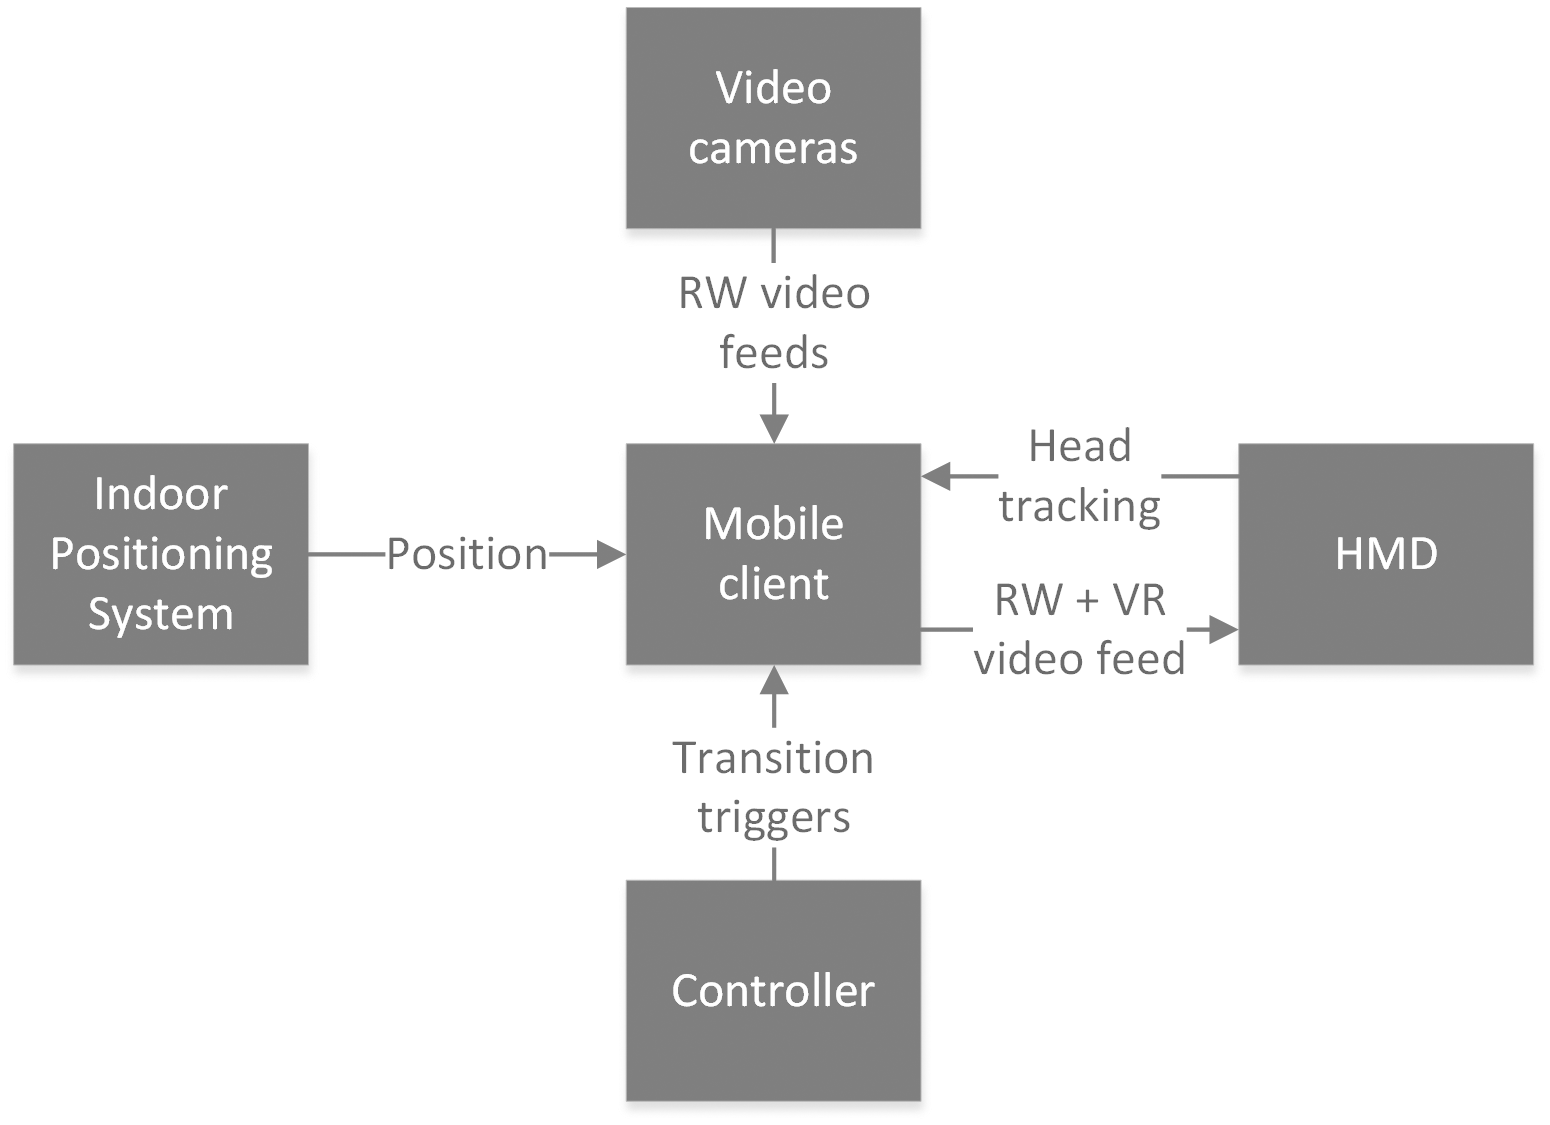
\includegraphics[width=.5\linewidth]{system-architecture.png}
		\caption{Overview of the Mirrorshades platform.}
		\label{systemarchitecture}
	\end{center}
\end{figure}

The HMD is imbued with video see-through functionality by the addition of cameras, to allow the user to see their RW environment. A controller held by the user allows them to trigger their view to switch between RW \& VR. The users' location within the cultural heritage site is tracked using an Indoor Positioning System (IPS). The mobile client that produces the graphical content delivered to the HMD can either be carried about the person (perhaps as a belt pack, or worn in a bag/satchel) or possibly be streamed from a powerful static computer to a lightweight mobile receiver carried about the person.

\textbf{***I think there needs to be some more explanation/diagram/picture of the system here before I start talking about the specifics of the implementation?}

%=========================================================================================================

\subsection{St Salvator's Chapel}

The stage upon which the Mirrorshades platform was designed \& developed to perform upon was St Salvator's chapel in St Andrews. Founded in 1450 but internally stripped of its medieval fittings during the Protestant Reformation (1517 - 1648), the chapel looks markedly different in the present day than it did upon its completion. An existing VR reconstruction of the chapel as it stood in the period 1450-1460 \& the marked differences between the internal appearance of the VR building \& the current building (including the replacement of the original stone roof with a wooden one \& drastically different dividing of the internal space) make this chapel an ideal candidate within the context of cultural heritage for the Mirrorshades PR system to be deployed.

\TwoFig{sallies-vrst/sallies-quad-real.jpg}{St Salvator's chapel, present day.}{sallies-quad-real.jpg}
       {sallies-vrst/sallies-quad-virtual.png}{St Salvator's chapel, reconstruction.}{sallies-quad-virtual.png}
       
This reconstruction project has virtually recreated St Salvator’s chapel as it was built and furnished for Bishop James Kennedy between 1450 \& 1460. The chapel was of the greatest significance for the new architectural ideas that it introduced into Scotland, at a time when Scotland was particularly open to external artistic influences. However, although the shell of the chapel survives and remains in use, it has lost its vault, its window tracery and its liturgical furnishings, and it now requires specialist skills to appreciate the quality of its original state. As with other reconstructions from the OVW group, the virtual St Salvator's chapel is a product of a collaboration between architectural \& art history \& computer science scholarship. On the combined evidence of a highly detailed late medieval inventory and of the architecture itself, it has been possible to show how the chapel was furnished internally with altars, choir stalls, lecterns, screens, stained glass and wall paintings. The virtual chapel is enhanced with lighting, sound and movement may be explored from a variety of physical and temporal locations through an avatar. The architectural, liturgical and spatial analysis allows our understanding of the history of the Chapel as a living building to be enormously enhanced by experiencing the building in its original context.

\TwoFig{sallies-vrst/sallies-real-toward-altar.jpg}{Looking towards the altar, present day.}{sallies-real-toward-altar.jpg}
       {sallies-vrst/sallies-virtual-toward-altar.png}{Looking towards the altar, reconstruction.}{sallies-virtual-toward-altar.png}

St Salvator's college was founded on 27 August 1450 by Bishop James Kennedy, who played a leading role in Scottish \& international politics. St Salvator’s was to be open to students who were prepared to live within the college. In this, St Salvator’s was the first college in Scotland to place the education of students so firmly at the heart of its role. It was dedicated for worship in 1460. The chapel is an aisle-less rectangle with a three-sided east apse. Deeply projecting three-stage buttresses define the bays, which are now capped by pinnacles of 1861–2. The windows which occupy the full space available between the buttresses, no longer reflect their original forms. The main entrance to the chapel was through a doorway in the second bay from the west of the south flank, which is covered by a vaulted porch between the buttresses. Two doorways on the north side presumably opened into a lost sacristy and treasury range.

The interior of the chapel is known to have been covered by a stone vault, which is assumed to have been of pointed barrel form with a decorative pattern of ribs, like the small vault over the south porch. The interior is now covered by an inappropriate timber roof.

\TwoFig{sallies-vrst/sallies-real-from-altar.jpg}{Looking from the altar, present day.}{sallies-real-from-altar.jpg}
       {sallies-vrst/sallies-virtual-from-altar.png}{Looking from the altar, reconstruction.}{sallies-virtual-from-altar.png}

St Salvator’s chapel is considered the first Scottish example of a church planned with an aisle-less rectangular main body terminating in a polygonal eastern apse, a type that was to have a long future for a range of Scottish church types. Such chapels were common in university colleges in France \& since Bishop Kennedy had a highly placed kinsman in the university of Paris and drew many ideas for the organisation of his college from that university’s constitution, it is reasonable to assume that he also drew some of his ideas for the architecture of his chapel from there. On this basis, St Salvator’s must be seen as an outstandingly important channel for the introduction into Scotland of new architectural ideas from France. The new architecture made a significant statement in its Scottish context. 

The reconstruction of the chapel involved both the mental reconstruction of modified and lost features, and the establishment of the range of ways in which buildings that represent a spirituality alien to modern students were intended to function. As such it offers an invaluable academic discipline for those involved in the reconstruction, providing eminently practical ways of testing theories and assumptions. It is then of the greatest value for conveying more widely the understanding that has been gained. The development of a PR system which enables comparison between the real and virtual chapel in the same time and place aims to further enhance the value of the reconstruction.

%=========================================================================================================

\section{Virtual Reality Head Mounted Displays}
The concept of virtual reality \& the associated head mounted displays that provide wide field of view, stereoscopic 3D graphics coupled with head tracking is currently experiencing a resurgence of interest \& investment, thanks largely to the advent of Oculus \& their Rift platform. Whilst the first head mounted computer display was created in the late 1960s by Ivan Sutherland~\cite{Rheingold1992}, it was not until the late 1980s \& early 1990s that VR began to be pushed to the consumer. Unfortunately, both the hardware \& software was not ready for consumer adoption at this time \& these systems failed to live up to the substantial hype of being a \textit{``revolutionary technology''} which \textit{``promises to transform society''} (see figure \ref{rheingold-virtual-reality.jpg}), resulting in the VR bubble bursting.

\begin{figure}[h]
	\begin{center}
		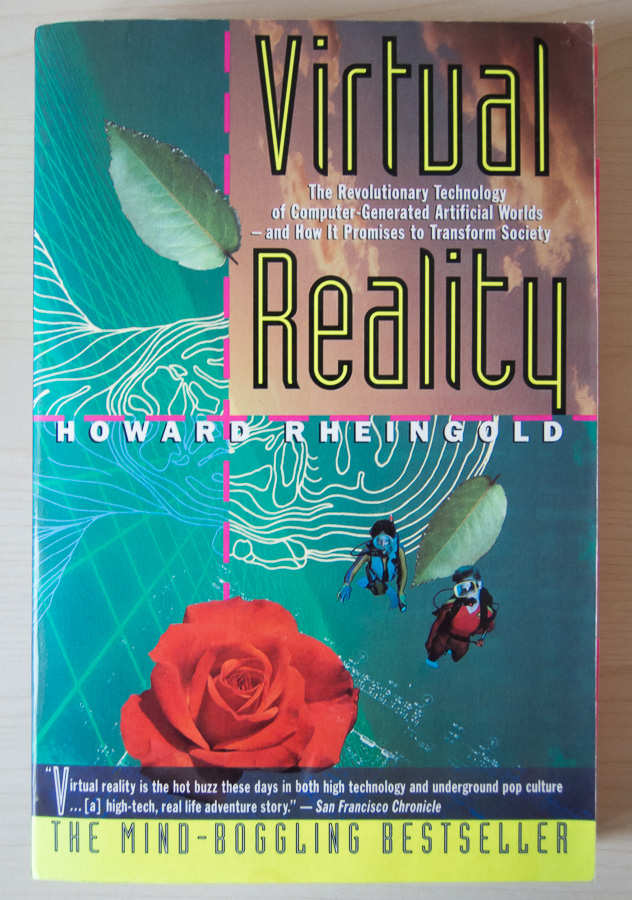
\includegraphics[width=0.4\textwidth]{rheingold-virtual-reality.jpg}
		\caption{Howard Rheingold's 1992 bestseller \textit{Virtual Reality}~\cite{Rheingold1992}.}
		\label{rheingold-virtual-reality.jpg}
	\end{center}
\end{figure}

Decades after this initial disappointment with consumer VR, Oculus now looks set to finally begin realising a successful consumer VR platform, thanks largely to the substantial advances in display technologies made during the past decade driven by the explosive popularity of smartphones \& tablets. Pre-Oculus HMDs predominantly made use of two separate microdisplays, one for each eye; Sutherland's original `Sword of Damocles' made use of two tiny CRT screens, whilst later HMDs made use of two OLED microdisplays. As the number of market applications for microdisplay technology was (\& continues to be) relatively small, there are limited models to chose from \& they command high prices when considering integration into a consumer device.

Oculus have taken a different approach for their Rift HMD. Instead of using two small displays, one for each eye, it uses a single larger display upon which two separate images are rendered, side-by-side. This approach has two distinct advantages compared to prior dual display techniques. Firstly, the complexity of the device is reduced, which effects both price, integration \& content development. Secondly, the cost of a single display in the 5"-7" range is drastically lower than the cost of a pair of microdisplays, thanks to the surging popularity of smartphones \& tablet computers. By making use of readily available displays intended for smartphone/tablet manufacturers, Oculus were able to bring their first Development Kit (DK1) to market for researchers \& enthusiasts at a price of only \$300, but still providing substantially wider FOV than the vast majority of existing HMDs (even those with vastly higher price points).

For comparison, examples of consumer-grade commercial HMDs that use the twin OLED microdisplay approach, the Sony HMZ-T1, which launched with a price of \textyen60,000 (\$800 at exchange rates of the time) \& its successor the HMZ-T2 which launched with a price of \textyen70,000 (\$900 at exchange rates of the time), provide $45\textdegree$ horizontal FOV/$51.6\textdegree$ diagonal \& no head tracking (intended primarily as a personal 3D cinema experience), whilst Oculus' DK1 provides more than $90\textdegree$ horizontal \& $110\textdegree$ diagonal FOV. Furthermore, the DK1 integrates a head tracking solution operating at a rate of 1kHz \& providing best in class accuracy. Combined with advances in both hardware \& software tasked with producing 3D graphics, the user experience of Oculus' HMD offerings is promising to finally deliver on the promises of 30 years previous.

The March 2014 acquisition of Oculus by Facebook\footnote{\url{https://www.facebook.com/zuck/posts/10101319050523971}} for \$2 billion\footnote{\url{http://www.theguardian.com/technology/2014/jul/22/facebook-oculus-rift-acquisition-virtual-reality}} \& Oculus partnership with Samsung, one of the world's leading display manufacturers, which has already led to the release of an innovative VR HMD that makes use of an existing smartphone as its display\footnote{\url{https://www.oculus.com/gear-vr/}}, lends hope that this wave of VR hype won't suffer the fate of its 90's cousin.

\textbf{***Maybe talk about what other HMDs there were actually available to me on the market? Vuzix 1200/900/whatever?}

%take bits from that youtube video from Samsung developers?

%=========================================================================================================

\subsection{The Oculus Rift DK1 \& Unity Game Engine}

The OVW group took delivery of an Oculus Rift DK1 from the first batch of units shipped to the EU, in August 2013. The immersive experience of using the DK1, thanks to its wide FOV, fast \& accurate head tracking, stereoscopic 3D \& novelty compared to traditional 2D displays, easily met the requirements of the display aspect of the Mirrorshades platform to exceed that of VTW in terms of user experience.

At this early stage in the DK1's release, the best supported software platform in terms of API provision \& integration was the Unity game engine. After experience with modifying the Second Life client with the VTW project, it was decided prudent to convert the OVW group's OpenSim model of St Salvator's chapel into a Unity compatible format, rather than embarking upon further modification to the Second Life client to support the DK1.

One deciding factor in this deliberation was the more stringent performance requirements for an enjoyable HMD experience compared to those of a traditional desktop/handhend display experience; when using a HMD such as the DK1, a high \& smooth framerate is required to avoid a kind of motion sickness referred to as `simulator sickness', with Oculus' official guidelines being for Rift applications to \textit{``run at a frame rate equal to or greater than the Rift display refresh rate''}\footnote{\url{http://static.oculus.com/sdk-downloads/documents/Oculus_Best_Practices_Guide.pdf}} which in the case of the DK1 is 60Hz. Due to the possibly ephemeral nature of Second Life content, where users are free to create, modify \& destroy content in real time, Second Life as a 3D platform suffers in terms of performance compared to game engines such as Unity due to not being able to exploit techniques such as occlusion culling~\cite{willmott:largecomplex} as these require an offline processing phase that depends upon environmental content to be static \& unchanging. The OVW group's experience in presenting Second Life/OpenSim content on a range of different hardware did not point to good odds of managing to render the St Salvator's chapel scene at 60fps, especially when considering that stereoscopic rendering introduces an overhead even when the total resolution of the two side-by-side images is no greater than the single monoscopic image. As Mirrorshades is a mobile application \& the computer producing the visuals may have to be worn \& carried by the user, the specification of this client may also be limited compared to those that the group has used in alternative deployments.

\textbf{***Some fps graphs of Second Life/OpenSim content with different hardware?}

%=========================================================================================================

\subsection{Modifying the DK1 for See Through Video}

The Oculus Rift DK1 covers the user's entire view, such that they cannot see any of their real world surroundings whilst wearing it, \& it does not feature any camera provision to allow a mediated view of the real world to be presented to the user. As such, it was necessary to modify the DK1 to provide such capability. When choosing cameras for this task, there were several desired ideal features;
\begin{itemize}
	\item resolution \& refresh rate that match (or exceed) those of the DK1,
	\item sensor aspect ratio that matches that of the DK1's display halves,
	\item combined lens focal length \& sensor dimension to provide wide FOV (ideally matching the FOV of the DK1),
	\item ease of integration with the Unity platform.
\end{itemize}

The PS3 Eye camera met most of these requirements. It's resolution is only 640x480 pixels, whilst each half of the DK1's display is 640x800 pixels, however unusually for a USB camera it is capable of running at 60fps (the refresh rate of the DK1). The aspect ratio of the 640x480 sensor is 4:3, which although not identical to the 5:4 aspect ratio of each eye's 640x800 `half' of the DK1 screen is closer than the 16:10 or 16:9 aspect ratio of a `widescreen' camera sensor. Furthermore, once dismantled to its bare PCB it features mounting holes for a standard S-mount (M12x0.5mm) lens mount commonly used for CCTV cameras, allowing alternative focal length lenses to be easily fitted.

A very early test with the PS3 Eye \& the DK1\footnote{\url{https://www.youtube.com/watch?v=tS0FGZxQzCU}} was performed by simply attaching a single unmodified PS3 Eye camera to the top of the DK1 (figure \ref{rift-pseye-ziptied.jpg}), with its stock lens set to its `wide' setting (75\textdegree, presumably diagonal, FOV\footnote{\url{http://uk.playstation.com/media/247868/7010571 PS3 Eye Web_GB.pdf}}). One purpose of this test was to explore the suitability of Unity's \texttt{WebCamTexture}\footnote{\url{http://docs.unity3d.com/ScriptReference/WebCamTexture.html}} feature for integrating the stream from a USB camera into a 3D application. In this early test, the mediated RW video stream was rendered to a small `floating' window that moved with the user's head (figure \ref{floating-webcam-window.png}), allowing the user to view both environments at once, with the real environment in their peripheral whilst they were attending to the virtual. Whilst an interesting concept, the decision was made to instead render the mediated RW stream to the full DK1 screen so as to allow the user to better observe their real environment thanks to the larger image \& higher resolution, with the small floating window likened more to the VTW approach of PR than an experience that allows true immersion in both environments. A second benefit of this switching approach is that it helps to mitigate any detrimental affect of latency in the camera image(s) not matching that of the virtual image(s).

\TwoFig{rift-pseye-ziptied.jpg}{First monoscopic see through hardware.}{rift-pseye-ziptied.jpg}
       {floating-webcam-window.png}{Early `floating' window see through video.}{floating-webcam-window.png}

A pair of PS3 Eye cameras were dismantled, removing their outer plastic housing \& stock lenses then fitting S-mount lens mounts. Ideally, the lenses used would provide the same FOV as the Rift itself is capable of displaying, such that the mediate RW stream from the cameras could be displayed at the full size of the Rift \& `match' the FOV of whatever virtual content would alternatively be displayed. However there is a trade off with lenses between focal length \& distortion; shorter focal lengths mean a wider FOV, however they also introduce more distortion which is not necessarily corrected by the shader that the Rift uses to compensate for the distortion of its own plastic lenses through which the image is viewed.

The PS3 Eye has a `1/4'' type' sensor which is only an indication of its true dimensions\footnote{\url{http://www.dpreview.com/glossary/camera-system/sensor-sizes}} \& as Sony has not published the actual dimensions of the sensor we adopt the typical 1/4'' type dimensions\footnote{\url{http://www.photoreview.com.au/tips/buying/unravelling-sensor-sizes}} of 4.5mm diagonal, 3.6mm horizontal, 2.7mm vertical for calculating FOV estimations. Empirical accounts of very short focal length S-mount lenses mounted to the PS3 Eye camera indicated that the distortion becomes very high beneath 2.1mm\footnote{\url{http://peauproductions.com/store/index.php?main_page=index&cPath=26_4}}. Table \ref{fov-table} gives the diagonal, horizontal \& vertical FOV of the widest readily available S-mount lenses.

\begin{table}
\begin{center}
\begin{tabular}{|c|c|c|c|}
\hline
Focal length (mm) & Diagonal FOV (\textdegree) & Horizontal FOV (\textdegree) & Vertical FOV (\textdegree) \\
\hline
2.5mm & 84    & 71.5 & 56.7 \\
2.1mm & 93.9  & 81.2 & 65.5 \\
2.0mm & 96.7  & 84   & 68 \\
1.9mm & 99.6  & 86.9 & 70.8 \\
1.8mm & 102.7 & 90   & 73.7 \\
1.7mm & 105.9 & 93.3 & 76.9 \\
\hline
\end{tabular}
\caption{FOV of various focal lengths resolving onto a 1/4'' type sensor.}
\label{fov-table}
\end{center}
\end{table}

Whilst 1.7mm lenses would provide almost identical FOV to the Rift's display (105.9\textdegree\ diagonal for the cameras, 110\textdegree\ diagonal for the Rift) the amount of distortion introduced would likely be of such an extent that the experience of viewing the mediate RW environment would be degraded more by distortion than by limited/non-matching FOV of longer focal length lenses, unless the lens' distortion was compensated in a separate stage. However, using a lens with a short enough focal length to provide a FOV as wide as the Rift isn't strictly necessary as, when wearing the Rift, the edges of the image presented to each eye are not necessarily visible to the user, especially if the Rift's adjustable distance from the eyes is adjusted such that it sits at its furthest position. Such adjustment is actually prudent, as using the Rift at its maximum extension from the eyes ensures maximum compatibility \& comfort with users \& also removes a variable between users compared to if each user is permitted to chose the extension themselves. Thus the choice of lens can be dictated by identifying the FOV required to fill the portion of the Rift's images that are visible when the headset is extended to its maximal position, rather than by matching the Rift's overall FOV, possibly allowing the use of lenses with focal length long enough that the distortion they introduce is not bad enough to require a separate correction phase.

Experiments revealed that with the DK1 set to its maximum extension, the area of the images visible to the user was wider than that provided by 2.5mm lenses (84\textdegree\ diagonal) when scaled correctly \& narrower than that provided by 2.1mm lenses (93.9\textdegree\ diagonal) when scaled correctly. Without easy availability of a lens with a focal length between 2.5mm \& 2.1mm it was decided to make use of the 2.1mm lenses. Figure \ref{lens-comparison-on-ps3eye-pcb.jpg} shows the 2.5mm lens (right) \& 2.1mm lens (left) mounted to the PS3 Eye PCBs via S-mount lens mounts, while figure \ref{fov-comparison-1.png} shows the FOV of the selected 2.1mm lenses scaled upon the wider FOV of the DK1's images - as previously mentioned, with the DK1 at its furthest extension, users cannot perceive the area outwith the mediated camera image.

\TwoFig{rift-clips-cameras/lens-comparison-on-ps3eye-pcb.jpg}{lens-comparison-on-ps3eye-pcb.jpg}{lens-comparison-on-ps3eye-pcb.jpg}
       {fov-comparison-1.png}{}{fov-comparison-1.png}

%{fov-comparison-2.png}{}{fov-comparison-2.png}

The PS3 Eye cameras were mounted to the DK1 by modifying the 3D printable sensor mount design released by the University of Southern California Institute for Creative Technologies\footnote{\url{http://projects.ict.usc.edu/mxr/diy/oculus-sensor-mount/}}. The modified mount comprised a base piece (figure \ref{clips.jpg}) that clips securely over the front of the DK1 \& a slotted plate (figure \ref{clips-hori-plate.jpg}) onto which the PS3 Eye cameras are mounted. These parts were 3D printed using a MakerBot Replicator 2X\footnote{\url{http://store.makerbot.com/replicator2x}} \& then combined using epoxy resin. The combination is shown attached to the DK1 by figure \ref{hori-1.jpg}. The slots in the slotted plate are spaced to match the mounting holes of the PS3 Eye PCB, such that the cameras can be attached by metal stand-offs (figure \ref{hori-2.jpg}) \& can then be easily moved left \& right to alter the distance between them to account for different interpupillary distances of different users. Figure \ref{hori-3.jpg} shows how one camera is mounted upside down to allow enough clearance for the PCBs to be moved close enough together to accommodate short interpuillary distances.

\begin{figure}[!htb]
    \centering
    \begin{minipage}{.32\textwidth}
        \centering
        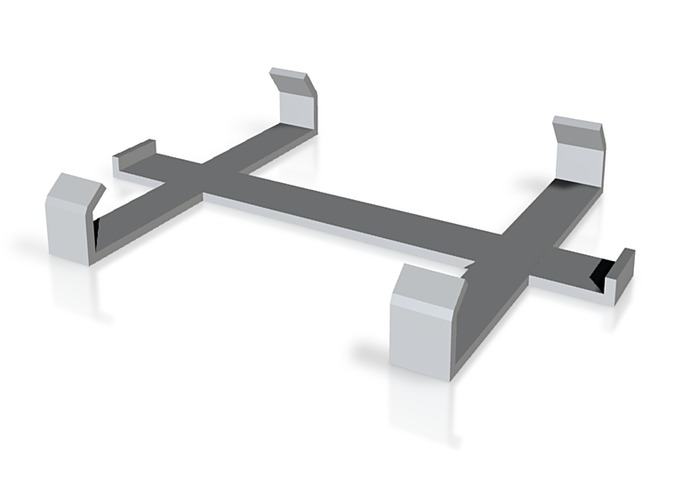
\includegraphics[width=\textwidth]{rift-clips-cameras/clips.jpg}
        \caption{bar}
        \label{clips.jpg}
    \end{minipage}%
    \hspace{.01\textwidth}
    \begin{minipage}{0.32\textwidth}
        \centering
        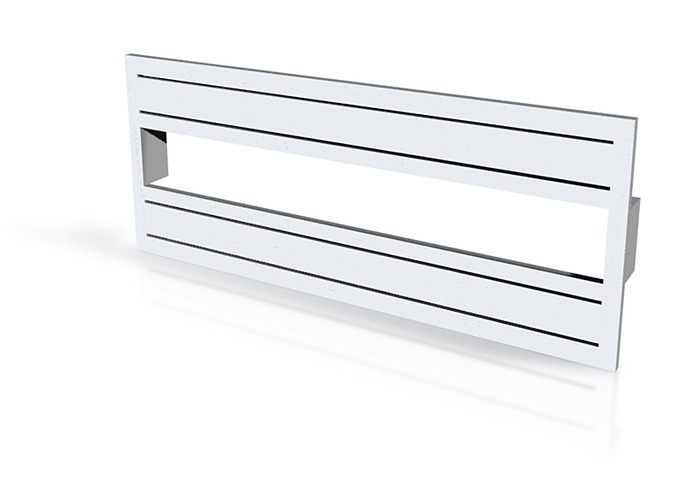
\includegraphics[width=\textwidth]{rift-clips-cameras/clips-hori-plate.jpg}
        \caption{foo}
        \label{clips-hori-plate.jpg}
    \end{minipage}%
    \hspace{.01\textwidth}
    \begin{minipage}{0.32\textwidth}
        \centering
        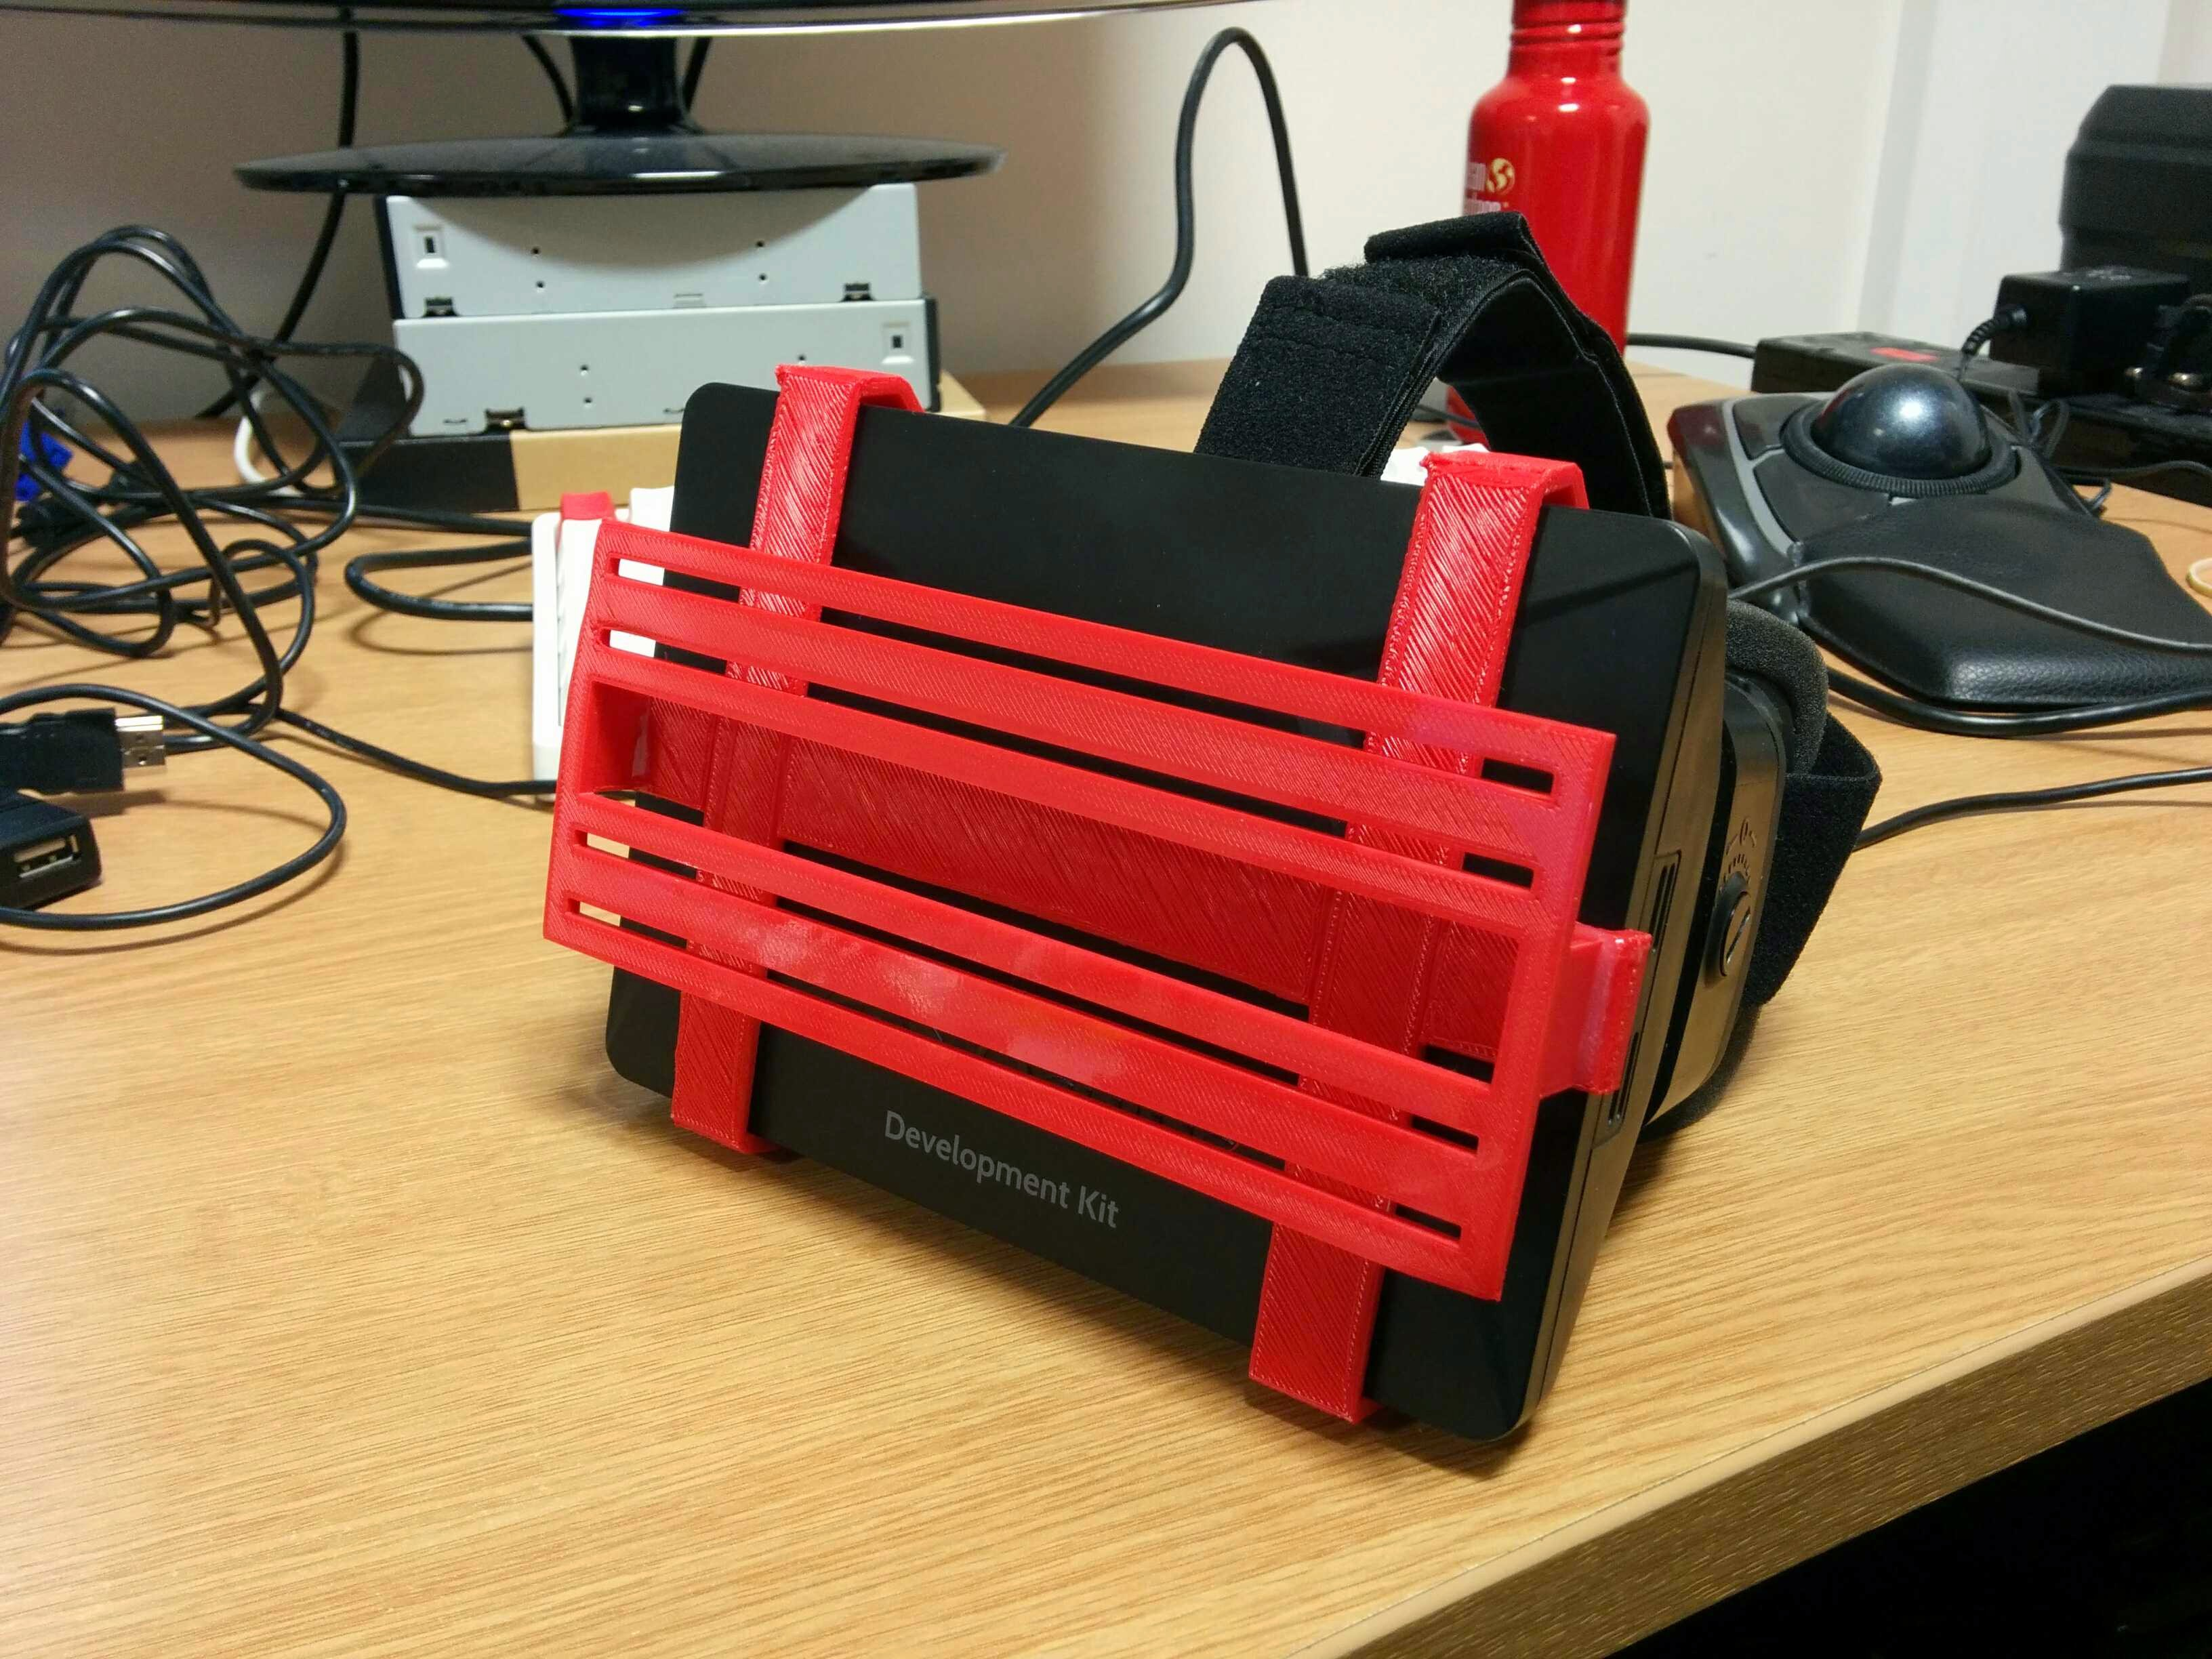
\includegraphics[width=\textwidth]{rift-clips-cameras/hori-1.jpg}
        \caption{baz}
        \label{hori-1.jpg}
    \end{minipage}
\end{figure}

\TwoFig{rift-clips-cameras/hori-2.jpg}{hori-2.jpg}{hori-2.jpg}
       {rift-clips-cameras/hori-3.jpg}{hori-3.jpg}{hori-3.jpg}

Although the initial integration test with a single PS3 Eye camera revealed easy accessibility of the camera within Unity, using two PS3 Eye cameras proved temperamental. Unity's \texttt{WebCamTexture} support identifies webcams via their `name' as provided by their driver. In the case of the PS3 Eye using the driver provided by Code Laboratories\footnote{\\url{https://codelaboratories.com/products/eye/driver/}} (this third party driver must be used as no official Windows driver is available with Sony only marketing the PS3 Eye for use with their PS3 console) an issue arises where both cameras present the same name to Unity \& the second camera overwrite the reference to the first, only allowing access to a single camera. Figure \ref{ps3-eye-unity-overwrite.png} shows this issue, that whilst Windows' device manager successfully identifies both cameras independently, Unity's \path{WebCamTexture.devices()} function returns a reference to only one (the \texttt{BisonCam, NB Pro} entry is the laptop's internal webcam). A partial solution to this issue was presented by a community provided Unity package\footnote{\url{http://tips.hecomi.com/entry/20130731/1375279561} (Japanese)}, which allowed the setup up to be successfully tested within a departmental building\footnote{\url{https://www.youtube.com/watch?v=oy5NqqDtkJ4}}.

\begin{figure}[h]
	\begin{center}
		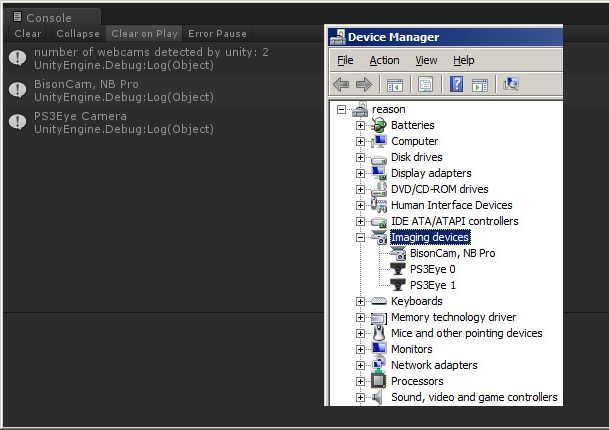
\includegraphics[width=.8\linewidth]{ps3-eye-unity-overwrite.png}
		\caption{Unity struggling with multiple PS3 Eye cameras.}
		\label{ps3-eye-unity-overwrite.png}
	\end{center}
\end{figure}

An oversight in the design of the camera mounts was realised by when William Steptoe later released details of his `AR Rift' project\footnote{\url{http://willsteptoe.com/post/66968953089/ar-rift-part-1}}. Although the DK1's overall screen has a resolution of 1280x800 in a `horizontal' 16:10 aspect ratio, each `half' of this screen as presented individually to each eye has a resolution of 640x800 in a `vertical' 4:5 aspect ratio. Thus to best match the aspect ratio of a 4:3 camera sensor, such as that of the PS3 Eye, to each half of the DK1's screen, that camera should be oriented in a portrait orientation rather than the landscape orientation employed by this project with the PS3 Eye cameras. Thus new mounting hardware was designed \& printed, by further modification of the USC's original 3D designs, allowing for vertical mounting of the PS3 Eye cameras. This new design is shown in figure \ref{clips-vert.jpg} (the recessed section in the centre of the clip allows for the heads of bolts to clear the front of the DK1) \& the assembled units are shown attached to the DK1 in figure \ref{vert-6.jpg}. Additionally soon after this point, the metal stand-offs that had been used to mount the camera PCBs to the clips (see figure \ref{vert-1.jpg}) were replaced with a combination of rubber washers \& threaded bolts (see figure \ref{vert-4.jpg}) both to reduce the discrepancy in the mediated RW images caused by the distance between the camera sensors \& the user's eyes (by reducing this distance) \& to allow for finer alteration of the orientation of the cameras.

\TwoFig{rift-clips-cameras/clips-vert.jpg}{clips-vert.jpg}{clips-vert.jpg}
       {rift-clips-cameras/vert-6.jpg}{vert-6.jpg}{vert-6.jpg}

\TwoFig{rift-clips-cameras/vert-1.jpg}{vert-1.jpg}{vert-1.jpg}
       {rift-clips-cameras/vert-4.jpg}{vert-4.jpg}{vert-4.jpg}

Unfortunately the PS3 Eye naming solution was temperamental at best \& two camera compatibility was frequently lost. It was decided prudent to therefore replace the PS3 Eye cameras with alternatives, rather than attempting to glean a solution to their reliable compatibility with Unity. Using Steptoe's project as a guide, a pair of Logitech C310\footnote{\url{http://www.logitech.com/en-gb/product/hd-webcam-c310}} cameras were sourced. Whilst the stated refresh rate of the C310 is only 30Hz, half that of the PS3 Eye, it supports a resolution of 1280x960, which is higher than that of the PS3 Eye \& of each half of the DK1's display. Thus the switch from the PS3 Eye cameras to the C310 represented a sacrifice in framerate, but an increase in resolution. Empirically the increase in resolution was however indiscernible, likely due to the effect of the DK1's optics reducing the visual acuity of its display, whilst the reduction in framerate was more prominently noticeable.

The C310 cameras received the same attention as the PS3 Eye cameras; they were dismantled \& outfitted with S-mount lens mounts. As the sensor in the C310 is also of the 1/4" type, the FOV provided by the 2.1mm lenses on the C310 cameras will be comparable to that of the same lenses mounted to the PS3 Eye cameras. Due to the lack of mounting holes present on the C310 PCB, the PCBs were set into a thin sheet of thermoplastic (figure \ref{thermoplastic.jpg}) which was then attached to the 3D printed clips with the same rubber washer \& threaded bolt arrangement as the PS3 Eye cameras. The assembled DK1 + dual C310 solution is shown by figures \ref{vert-7.jpg} (3/4 view), \ref{middle.jpg} (profile view) \& \ref{right.jpg} (detail view).

\TwoFig{rift-clips-cameras/thermoplastic.jpg}{thermoplastic.jpg}{thermoplastic.jpg}
       {rift-clips-cameras/vert-7.jpg}{vert-7.jpg}{vert-7.jpg}

\TwoFig{rift-clips-cameras/middle.jpg}{middle.jpg}{middle.jpg}
       {rift-clips-cameras/right.jpg}{right.jpg}{right.jpg}



\TwoFig{latency/vid1.jpg}{vid1.jpg}{vid1.jpg}
       {latency/vid2.jpg}{vid2.jpg}{vid2.jpg}

\TwoFig{latency/vid3.jpg}{vid3.jpg}{vid3.jpg}
       {latency/vid4.jpg}{vid4.jpg}{vid4.jpg}



\begin{figure}[h]
    \begin{center}
    \begin{minipage}{.32\textwidth}
        \begin{center}
        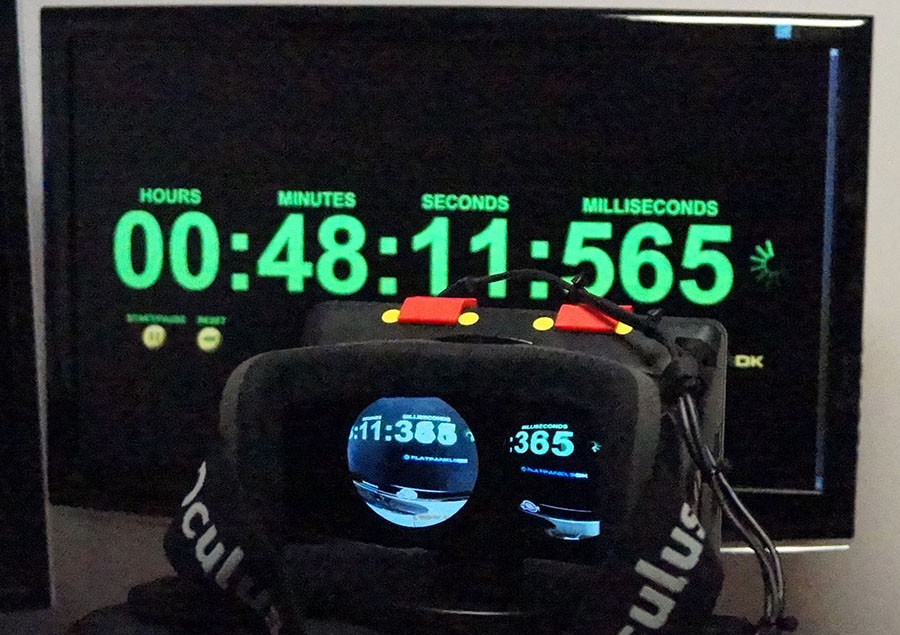
\includegraphics[width=\textwidth]{latency/still1.jpg}
        \caption{still1.jpg}
        \label{still1.jpg}
        \end{center}
    \end{minipage}%
    \hspace{.01\textwidth}
    \begin{minipage}{.32\textwidth}
		\begin{center}
        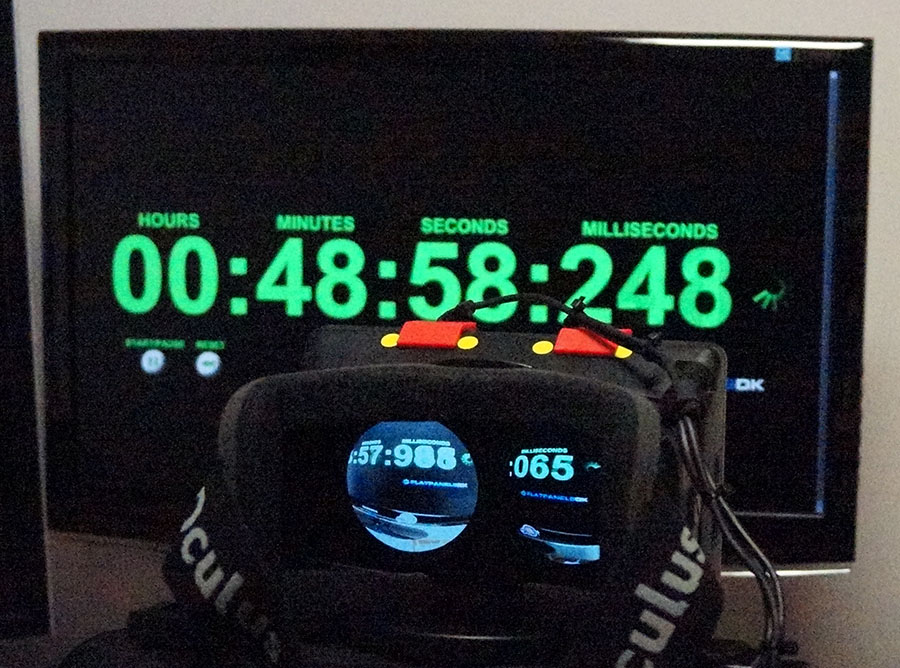
\includegraphics[width=\textwidth]{latency/still2.jpg}
        \caption{still2.jpg}
        \label{still2.jpg}
        \end{center}
    \end{minipage}%
    \hspace{.01\textwidth}
    \begin{minipage}{.32\textwidth}
        \begin{center}
        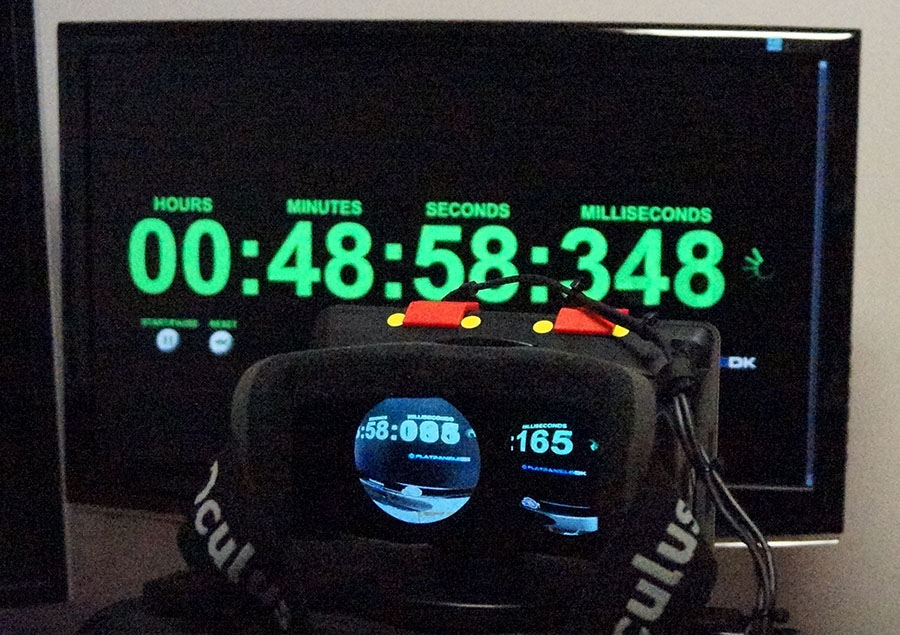
\includegraphics[width=\textwidth]{latency/still3.jpg}
        \caption{still3.jpg}
        \label{still3.jpg}
        \end{center}
    \end{minipage}
    \end{center}
\end{figure}

%=========================================================================================================

\section{Indoor Positioning Systems}

For outdoor applications, GPS represents a suitable solution for the vast majority of position tracking requirements. Global coverage \& the ability to scale accuracy as required, from many metres with a basic GPS receiver such as those integrated into smartphones, to a few metres with SBAS augmentations \& further to as little as 10cm with the deployment of Differential GPS (DGPS) beacons, has led to GPS occupying the role of the `go to' solution where position tracking is required for an outdoor application. For indoor applications however, there is no single technology or solution that provides similar coverage or suitability as GPS does outside: a large number of different technologies have been employed to produce Indoor Positioning Systems (IPS), which are summarised in figure \ref{mautz-table.png}.

\begin{figure}[h]
	\begin{center}
		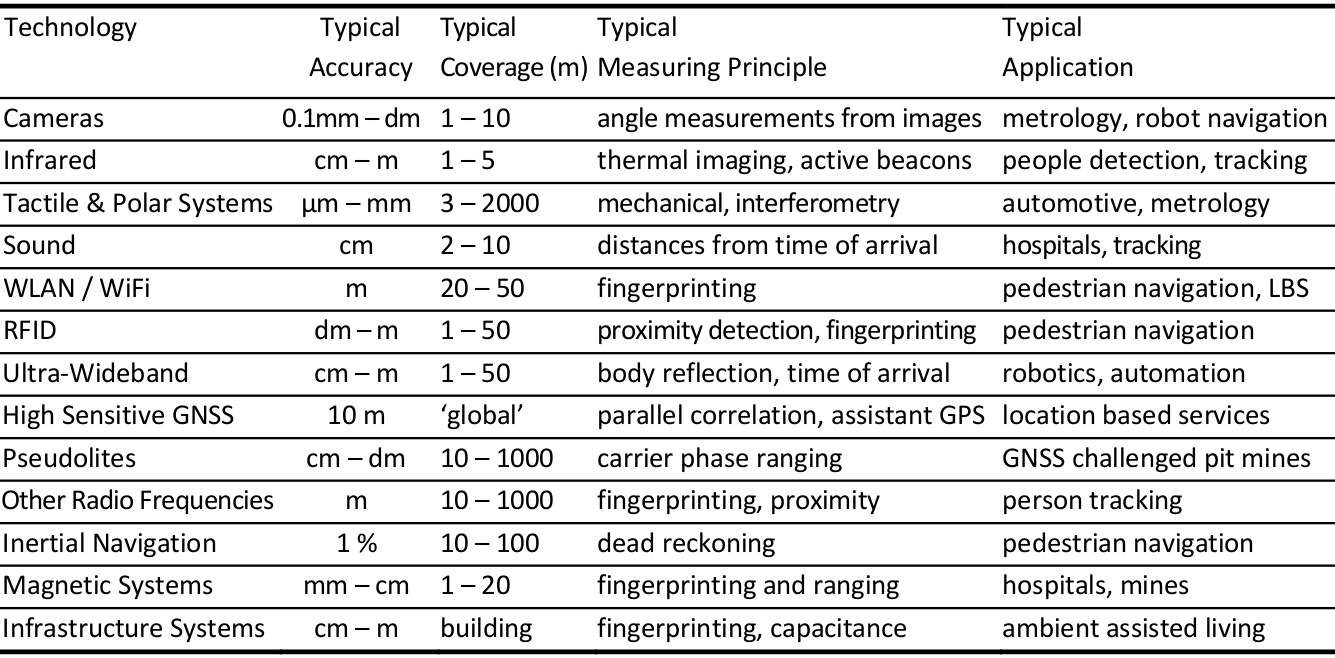
\includegraphics[width=\linewidth]{mautz-table.png}
		\caption{Overview of IPS technologies, from~\cite{Mautz2012}.}
		\label{mautz-table.png}
	\end{center}
\end{figure}

Because of this diversity in technology, with different IPS solutions covering various swathes of the continuums of accuracy \& coverage (see figure \ref{Mautz-000.png}), introducing a host of performance \& suitability considerations, it is necessary to carefully consider the requirements of the application (see figure \ref{Mautz-003.png}) \& then choose the best suited of the many different IPS approaches. Unsurprisingly, selection of a particular IPS usually leads to balancing these requirements in a trade-off, as each of the challenges of indoor positioning effects each technology more or less than others~\cite{Mautz2009}.

\TwoFig{Mautz-000.png}{IPS technologies plotted against their accuracy \& coverage, from~\cite{Mautz2012}.}{Mautz-000.png}
       {Mautz-003.png}{Requirements parameters of IPS, from~\cite{Mautz2012}.}{Mautz-003.png}

%=========================================================================================================

\subsection{IPS Requirements for Mirrorshades}
The positional accuracy of the IPS used for the Mirrorshades platform needs to be substantially higher than that of the GPS solution used for VTW. As a pedestrian application wherein the user walks through doorways (whether real or virtual) \& observes multiple rooms within a building, it is necessary to achieve a level of accuracy that allows, for example, reliably discerning between adjacent rooms, between a doorways \& their surrounding walls \& for approximating position within rooms \& corridors.

Coverage required depends largely upon the size of the cultural heritage site that Mirrorshades is deployed to. However it is prudent to select an IPS that can scale quite arbitrarily from small scenarios (perhaps of a small village church) to substantially larger scenarios (such as a cathedral similar to that at St Andrews), such that the suitability of the platform isn't restricted to sites of particular sizes.

A high update frequency is not especially important to Mirrorshades. The envisaged style of interaction is one wherein users walk relatively slowly through the environments, as they wish to observer \& take in their surroundings. Updates in the range of several hz will be sufficient, especially if users are attending more to their real environment than the equivalent virtual environment when actively moving around (which is to be encouraged, as one cannot walk through a RW obstacle as one can a VR one). Similarly, low latency is not critical. Even if the IPS takes a few seconds to `catch up' with the user, because the user is committed to a deliberate study \& comparison of their real \& virtual surroundings they are not going to be foiled in their task if they find they have to wait momentarily when switching from real to virtual views.

Cost represents a more concrete restriction for Mirrorshades, as the costs of installing \& using different IPS range drastically. For example, an IPS that locates users via propagation modelling/empirical fingerprinting/pathloss of WiFi signals can make use of existing WiFi infrastructure installed in a building \& use nothing more expensive than a smartphone carried by the mobile user. Conversely, using a motion capture suit as an IPS solution will incur substantial costs for each suit, with additional costs for the supporting infrastructure. In a similar vein to the vision of Mirrorshades, an existing project combined the Oculus Rift HMD with an Xsens MVN motion capture suit, allowing participants to walk around a virtual environment of the same layout \& dimensions as their real environment\footnote{\url{https://www.youtube.com/watch?v=LtMfrkRqlRs}}, but without any video see-through of the real environment. The use of a motion capture suit allowed extremely accurate positional tracking, however as a \textit{``complete standard Xsens MVN system is available at around \euro{}50,000''}\footnote{Personal correspondence with Xsens EMEA Entertainment Business Manager.} \& requires a not insubstantial setup phase of the participant donning the suit, it is unsuitable for a virtual heritage scenario where budget is likely to be substantially more limited \&  where visitors are unlikely to be willing to don a complex motion capture suit in order to explore the site. To illustrate a real world comparison of the trade off between costs, accuracy, frequency, etc. of different IPS technologies, considering the departmental building shown by \ref{jack-cole-splodges-black.png}, \textit{``To cover ground floor and have room level accuracy in each room + tracking in the corridors, the cost would be ca. \$25,000''}\footnote{Personal correspondence with Sonitor Technologies Vice President Sales and Business Development EMEA \& APAC.} for a commercial ultrasonic IPS.

Reliance upon deployed infrastructure such as beacons \& markers needs to be avoided for Mirrorshades, as most cultural heritage sites will not allow the installation of any such infrastructure into the site/environment, or may only allow strictly temporary infrastructure to be deployed. Approaches that require extensive infrastructure to be deployed, or for which the deployment \& calibration phase of infrastructure is long \& thus not suitable for temporary deployments, are therefore unusable. Similarly, intrusiveness of the IPS used for Mirrorshades needs to be considered such that the IPS does not drastically affect the user's ability to observe the real \& virtual sites around them.

Robustness of all aspects of a virtual heritage system is critical for enjoyment \& beneficial experience by the user. Visitors to a cultural heritage site, especially if they are only visiting for a short period of time in passing, are not going to be pliant to waiting for a malfunctioning virtual heritage system to right itself. Furthermore, many virtual heritage systems are installed in situations in which the on-site staff do not have the technical knowledge or experience to troubleshoot \& repair them, so these systems must be robust enough to continue successful operation for extended periods of time without intervention by knowledgeable administration.

%http://www.memsic.com/wireless-sensor-networks/MCS-KIT410CA
%8x Crickets
%GBP1850
%email from Willow.co.uk

%=========================================================================================================

\subsection{PlayStation Move}

An initial technology investigated for suitability as an IPS for use with Mirrorshades was PlayStation Move (PSMove), a game controller platform released by Sony for use with their PlayStation 3 console. The platform comprises a hand held controller which contains inertial sensors \& has a plastic sphere on its end that is illuminated from within by a RGB LED. A bundled webcam, the PlayStation Eye (referred to as `PS3 Eye', `PS3Eye' \& `PSEye' among the literature \& community) uses vision tracking to track the controller's position in relation to the camera. Through use of the PSMove API~\cite{Perl2012}, the PSMove platform can be used by a regular computer, by making use of the OpenCV\footnote{\url{http://opencv.org/}} computer vision project.

Whilst the PSMove has been used successfully for pedestrian position tracking in previous projects, included those that used an Oculus Rift HMD\footnote{\url{http://projects.ict.usc.edu/mxr/blog/project-holodeck-wows-in-dublin/}}, it quickly became apparent when auditioning the platform that it only performs reliably when in very dimly lit conditions. Even the relatively dim scene shown by figure \ref{psmove-screenshot.png} (see also ) represented too much ambient light for reliable tracking, so the suitability of the platform for use at a cultural heritage site was removed.

\begin{figure}[h]
	\begin{center}
		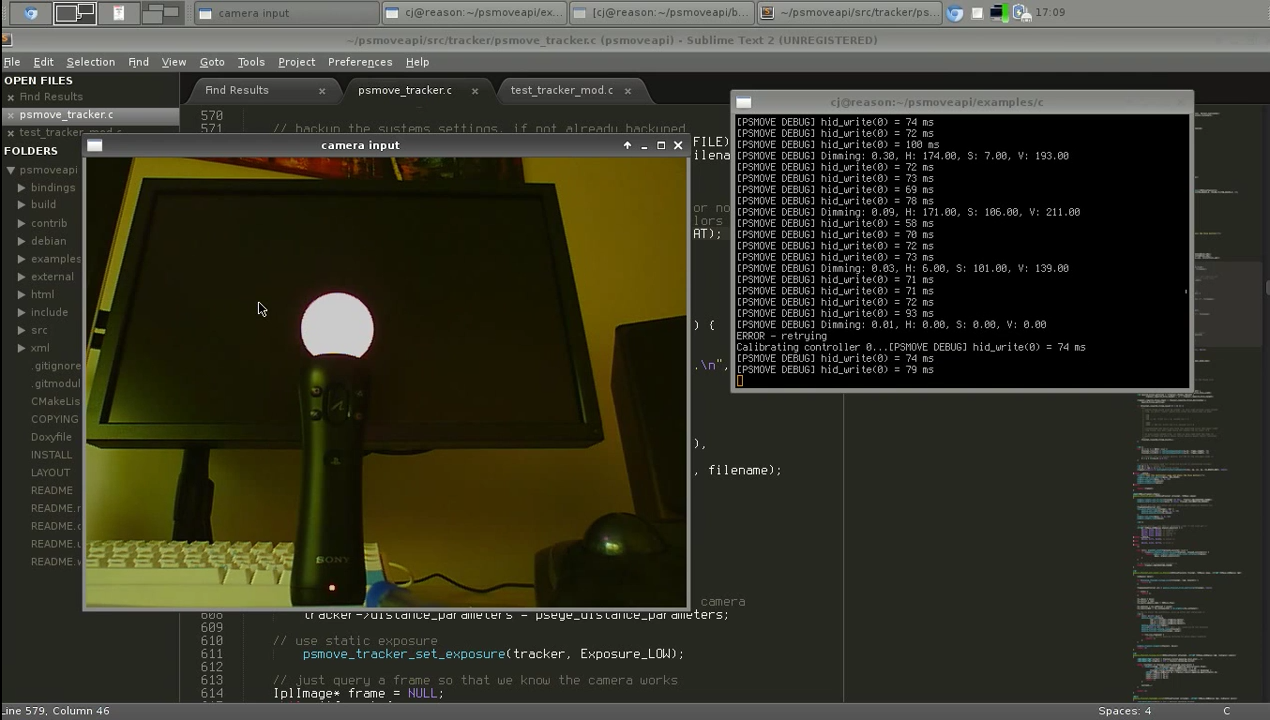
\includegraphics[width=.8\linewidth]{psmove-screenshot.png}
		\caption{PSMove failing to locate even in dim conditions.}
		\label{psmove-screenshot.png}
	\end{center}
\end{figure}

%=========================================================================================================

\subsection{Indoor Atlas}

During the evaluation phase of different IPS \& their suitability to the envisaged Mirrorshades platform, Finnish startup IndoorAtlas\footnote{\url{https://www.indooratlas.com/}} released the first public beta of their indoor positioning technology that uses the magnetometers found in smartphones to locate a user within a magnetic `fingerprint' of a particular building, taking inspiration from animals, such as the spiny lobster, that are able to determine their position in addition to their direction from the Earth's magnetic field~\cite{Boles2003}. A spin out from research at the University of Oulu in 2009~\cite{Haverinen2009,Haverinen2009a}, with a similar project undertaken by Media Lab researchers in 2011~\cite{Chung2011}, IndoorAtlas exploits how the Earth's magnetic field is distorted by both natural \& man-made sources. Indoors, these distortions come from building materials, especially in structures employing a framework of metal beams, but also from electrical cabling, HVAC ducting, etc. By recording a map of these distortions in an offline mapping phase, producing a fingerpint of the magnetic field around a building, the location of a user can be deduced by comparing the readings from their smartphone's magnetometer to this fingerprint in real time.

IndoorAtlas promised to be a good match for the IPS requirements of the Mirrorshades platform. In particular, the lack of dependence upon any deployed infrastructure such as ultrasound beacons or visual tracking targets suits the deployment area of Mirrorshades well, as most cultural heritage sites will not be amenable to the deployment of such hardware. Furthermore, the reliance upon only a smartphone held by the user means that coverage is only limited by the area that has prior been mapped in an offline mapping phase, allowing the positioning to scale to arbitrarily large indoor cultural heritage sites. This dependence upon only a smartphone also meets the low cost requirement of the Mirrorshades platform, as mid to high end smartphones with sensitive magnetometers can be purchased for just a few hundred dollars.

The major concern at this point was whether the building materials employed in the construction of cultural heritage sites such as chapels, castles \& cathedrals would create great enough distortions to the Earth's magnetic field for IndoorAtlas to provide its boasted accuracy (which would be sufficient to discern between adjacent rooms, between doorways \& their surrounding walls \& estimate position within rooms \& corridors). These building materials are largely various types of stone, along with wood, a far cry from the metal framework that permeates most modern buildings. Whilst initial tests of the IndoorAtlas beta technology within a departmental building\footnote{\url{https://www.youtube.com/watch?v=l-eIvzpScRs}}\footnote{\url{https://www.youtube.com/watch?v=9hc2zEeQJXQ}} of roughly 40m \& 30m tall were promising, this was a modern building with a steel beam structure \& an abundance of computing infrastructure \& its associated cabling \& cooling provision. Figure \ref{jack-cole-splodges-red.png} shows the results of one of these tests, with each red dot representing a position reported by the IndoorAtlas platform while walking around the building at a slow walking pace ($<1$ms$^{-1}$, akin to how a visitor to a cultural heritage site might walk.

\TwoFig{jack-cole-splodges-red.png}{Positions reported by IndoorAtlas.}{jack-cole-splodges-red.png}
       {jack-cole-indooratlas-routes.png}{Route mapped during offline phase.}{jack-cole-indooratlas-routes.png}

It should be noted that the IndoorAtlas technology only reports positions upon routes that have been previously mapped in an offline mapping phase; for the test results shown by figure \ref{jack-cole-splodges-red.png}, this offline mapping phase comprised walking the route shown by the thick black line in figure \ref{jack-cole-indooratlas-routes.png} several times. In the following test, had the user deviated from this route, IndoorAtlas would still have reported them as being somewhere upon it; it would not attempt to extrapolate their position into unmapped territory. This is presumably because the scale of distortions in the Earth's magnetic field is quite fine grained, supported by the fact that many of the black dots are less than a meter apart, thus extrapolation would not fair well. This is an important aspect to take into account when performing the offline mapping phase, as one must map sufficient paths to cover all possible places \& routes that a user may walk. For locations comprised mainly of corridors \& small rooms, this is not an issue, however for a location that contains a large open space in which the user is free to meander, a more involved mapping process in which the entire space is systematically covered by back \& forth routes that progress across the space is required.

Initial testing of IndoorAtlas at St Salvator's chapel proved surprisingly successful, with the platform able to track the smartphone accurately throughout the building even without any obvious overbearing metal content in the structure or its furnishings. Figure \ref{sallies-splodges-red.png} shows the set of positions reported by the IndoorAtlas platform whilst walking throughout the chapel, which is roughly 30m across, after an offline mapping phase that mapped the routes shown in figure \ref{sallies-indoor-atlas-routes.png}.

\TwoFig{sallies-splodges-red.png}{Preliminary testing of IndoorAtlas in St Salvator's chapel.}{sallies-splodges-red.png}
       {sallies-indoor-atlas-routes.png}{Routes mapped during offline phase.}{sallies-indoor-atlas-routes.png}

Upon closer inspection of the building, metal grating that runs along the ground along the central aisle, representing much of the horizontal movement in figure \ref{sallies-splodges-red.png} \& shown in figure \ref{DSCN0172.jpg} \& figure \ref{DSCN0174.jpg} in detail, which also extends to the open area in front of the altar as shown in figure \ref{DSCN0175.jpg}, may explain this unexpectedly high performance, however in other areas such as when walking to either side of the altar (far right of figures \ref{sallies-splodges-red.png} \& \ref{sallies-indoor-atlas-routes.png}) there were no obvious sources, as seen in figure \ref{DSCN0176.jpg}, of magnetic interference to account for the maintained accuracy. Possible less obvious explanations could be the ferromagnetic properties of certain types of stone used in the building's construction \& the presence of electrical lighting \& audio systems installed into the chapel (loudspeaker \& light fixture visible in figure \ref{DSCN0177.jpg}), which presumably make use of electrical cables routed throughout the building.

\begin{figure}[h]
    \begin{center}
    \begin{minipage}{.32\textwidth}
        \begin{center}
        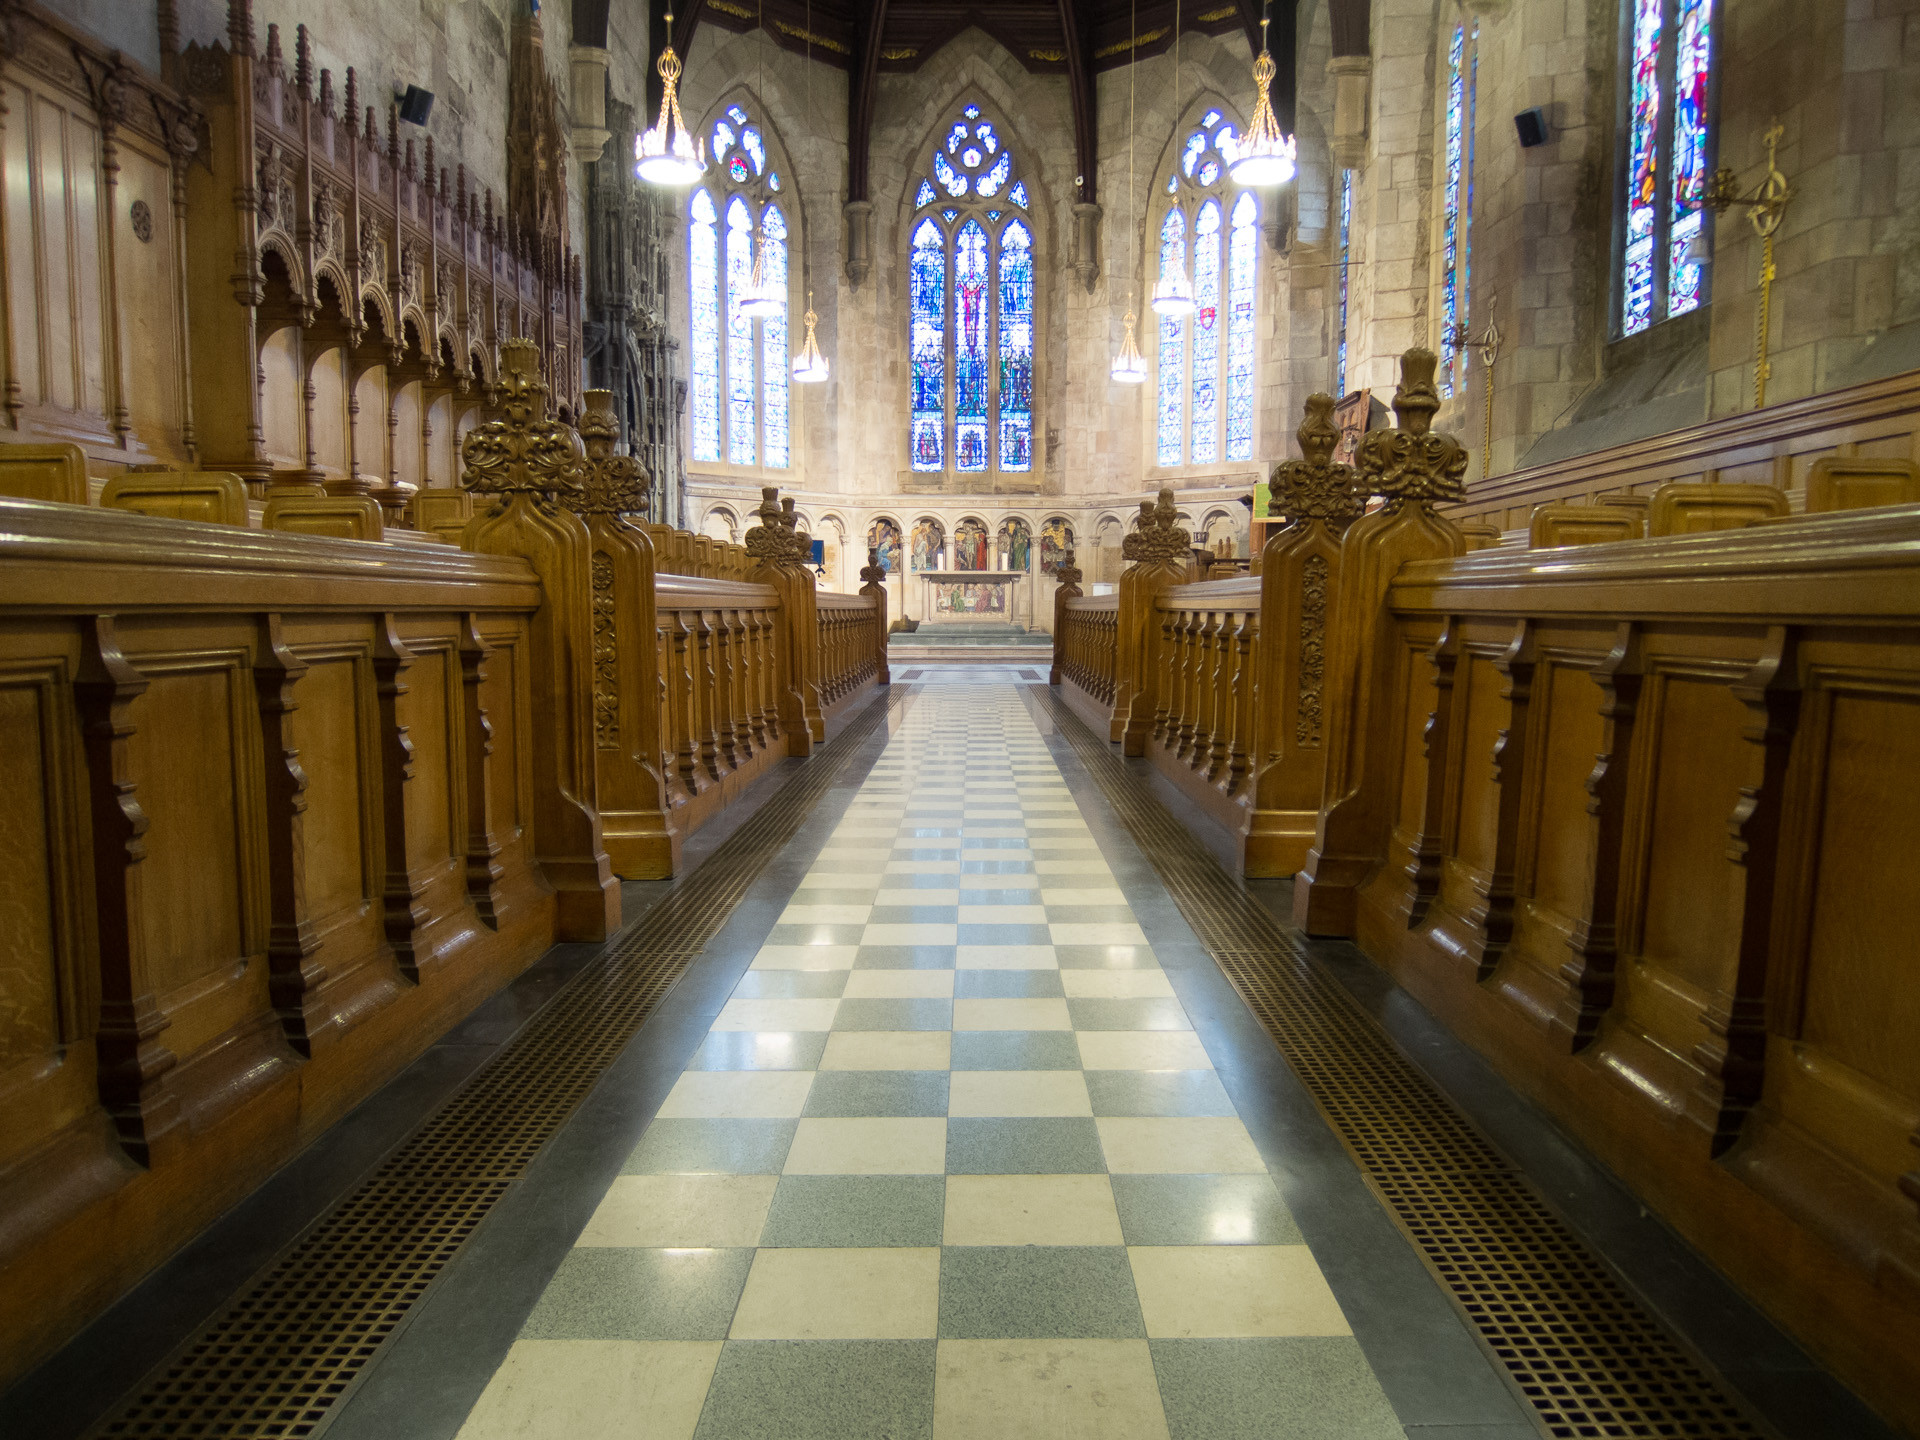
\includegraphics[width=\textwidth]{Sallies-photos/DSCN0172.jpg}
        \caption{Chapel aisle, flanked by gratings.}
        \label{DSCN0172.jpg}
        \end{center}
    \end{minipage}%
    \hspace{.01\textwidth}
    \begin{minipage}{.32\textwidth}
		\begin{center}
        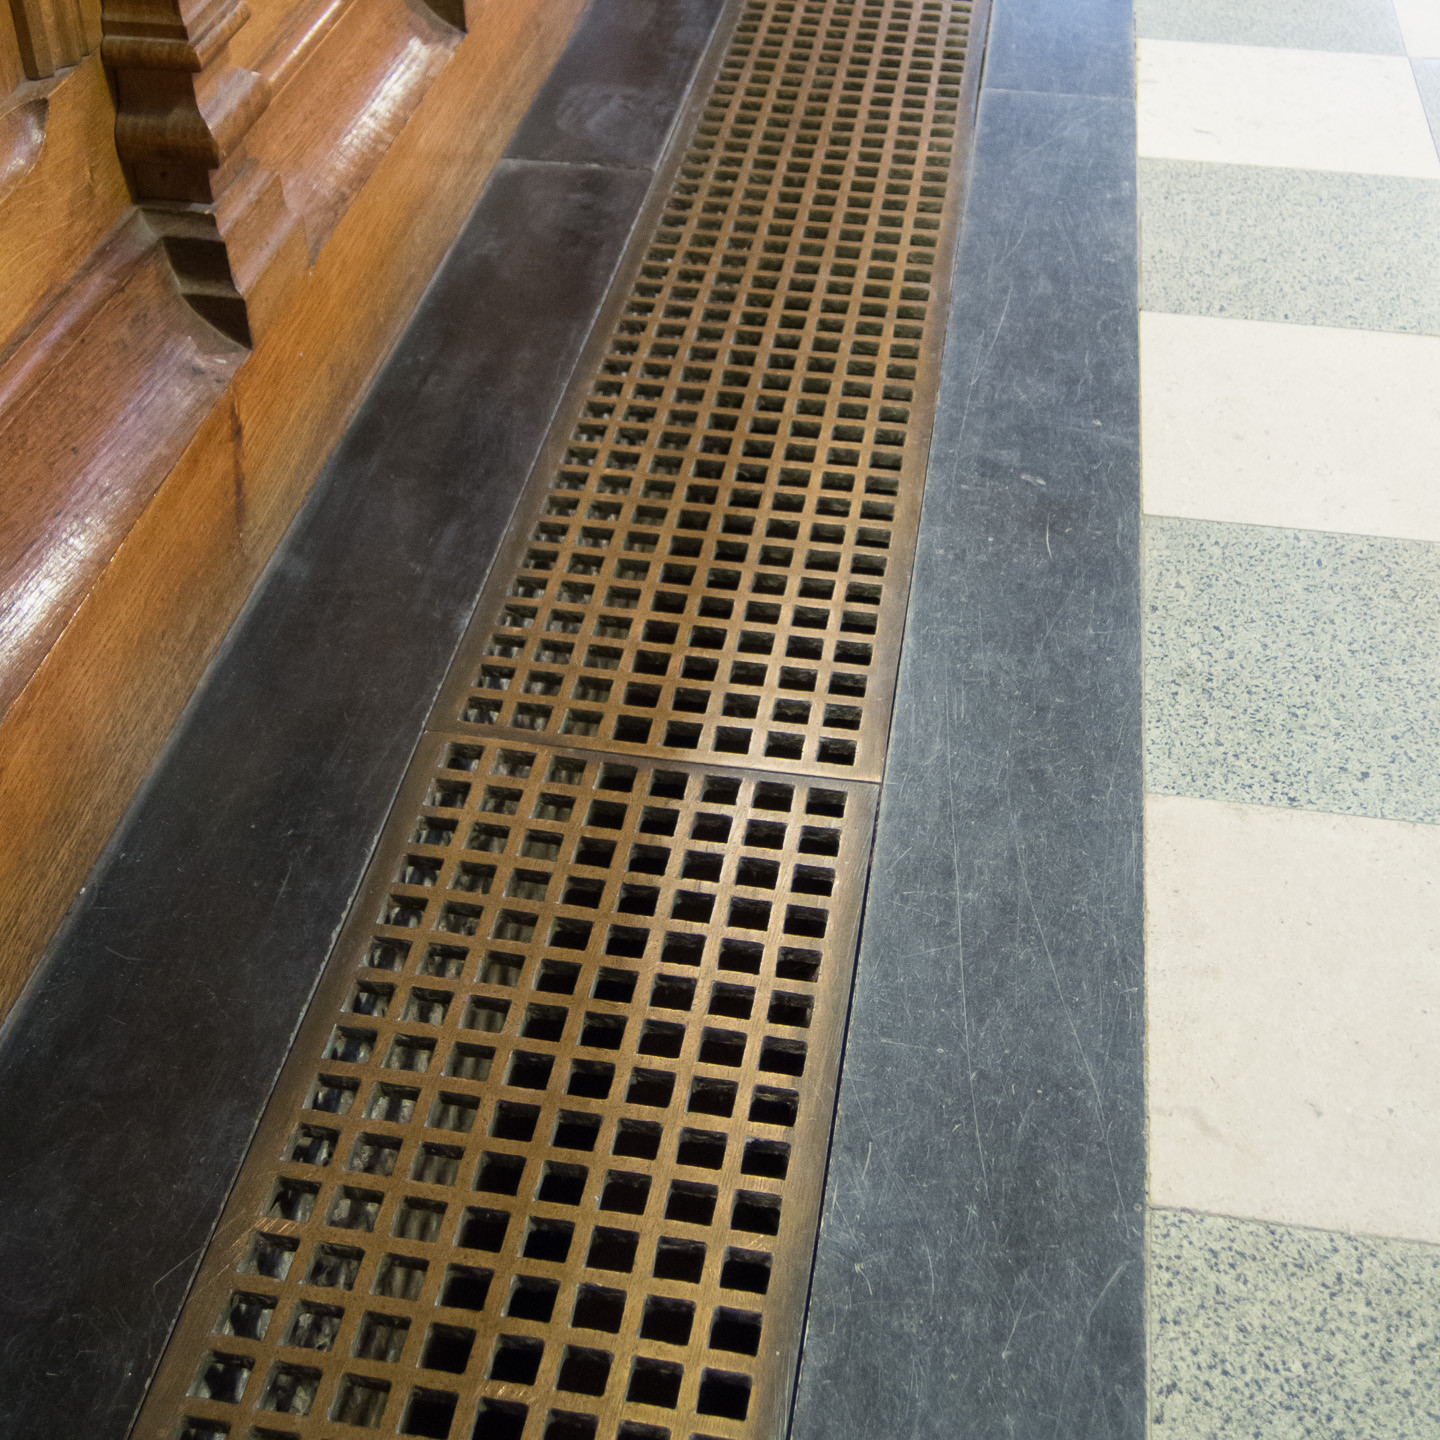
\includegraphics[width=\textwidth]{Sallies-photos/DSCN0174.jpg}
        \caption{Grating detail.}
        \label{DSCN0174.jpg}
        \end{center}
    \end{minipage}%
    \hspace{.01\textwidth}
    \begin{minipage}{.32\textwidth}
        \begin{center}
        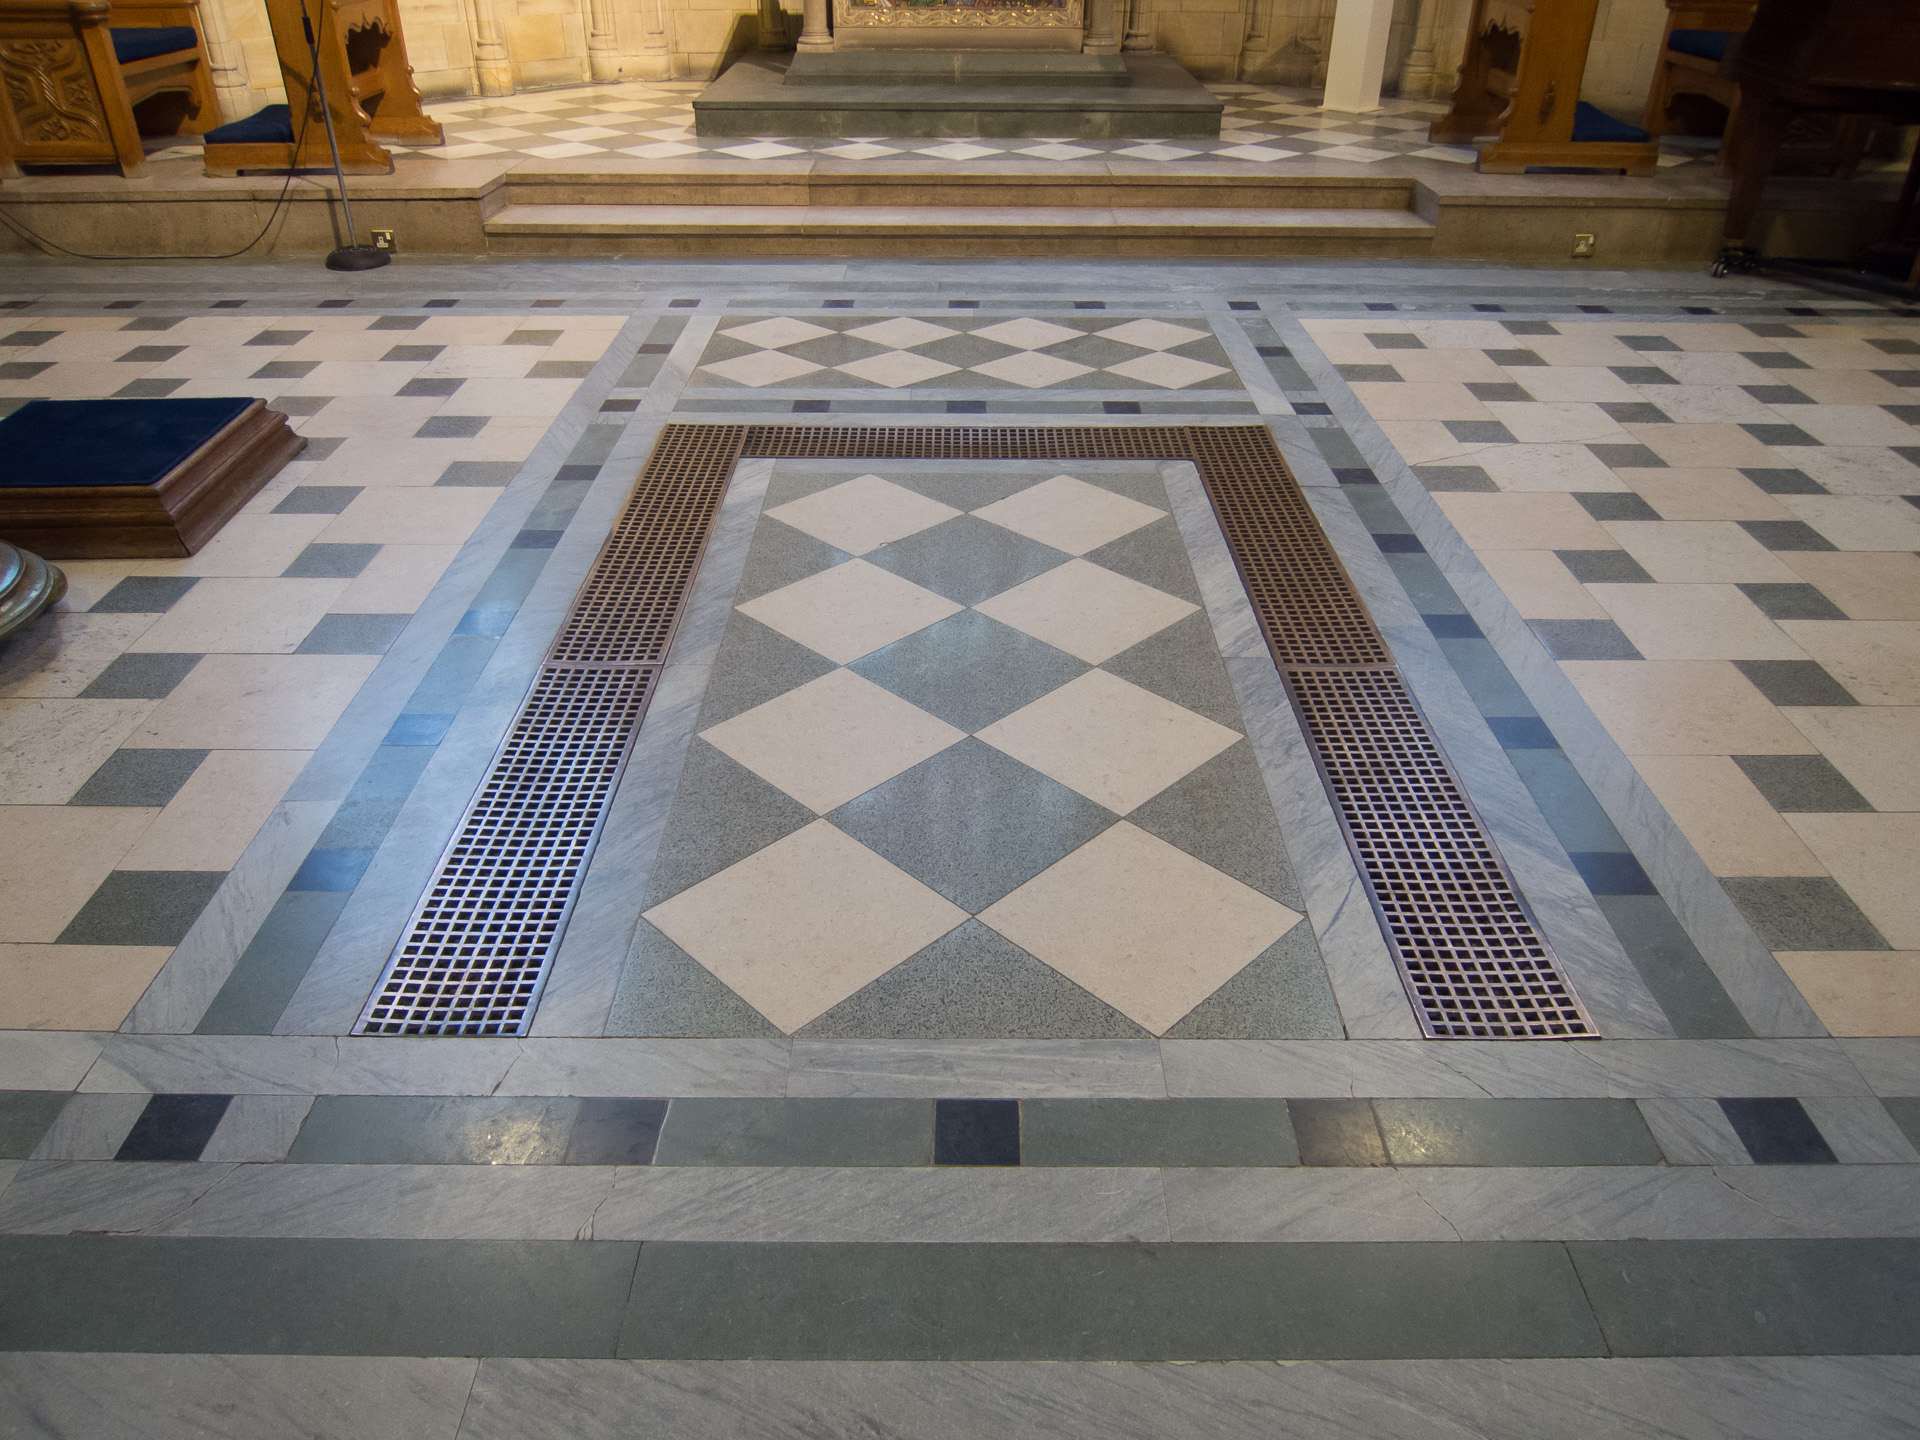
\includegraphics[width=\textwidth]{Sallies-photos/DSCN0175.jpg}
        \caption{Gratings before altar.}
        \label{DSCN0175.jpg}
        \end{center}
    \end{minipage}
    \end{center}
\end{figure}

\TwoFig{Sallies-photos/DSCN0176.jpg}{No obvious metal around altar.}{DSCN0176.jpg}
       {Sallies-photos/DSCN0177.jpg}{Loudspeaker \& electric light fixture.}{DSCN0177.jpg}

%=========================================================================================================

\section{Mobile Client}

Talk about trying Oculus on Android (ODROID) \& how now Samsung Gear VR would be ideal, but yolo laptop in a bag. Photo of ODROID/screencap of (\& link to) video showing Rift working (at least tracking) with ODROID?

Talk about ease of Unity integration with Oculus at the time (UE4 wasn't really on the scene?).

%=========================================================================================================

\subsection{Implementation}
Figure \ref{experimentalimplementation} presents an overview of the implementation of the Mirrorshades platform design for use in the chapel investigations.

\begin{figure}[h]
	\thispagestyle{empty}
	\begin{center}
		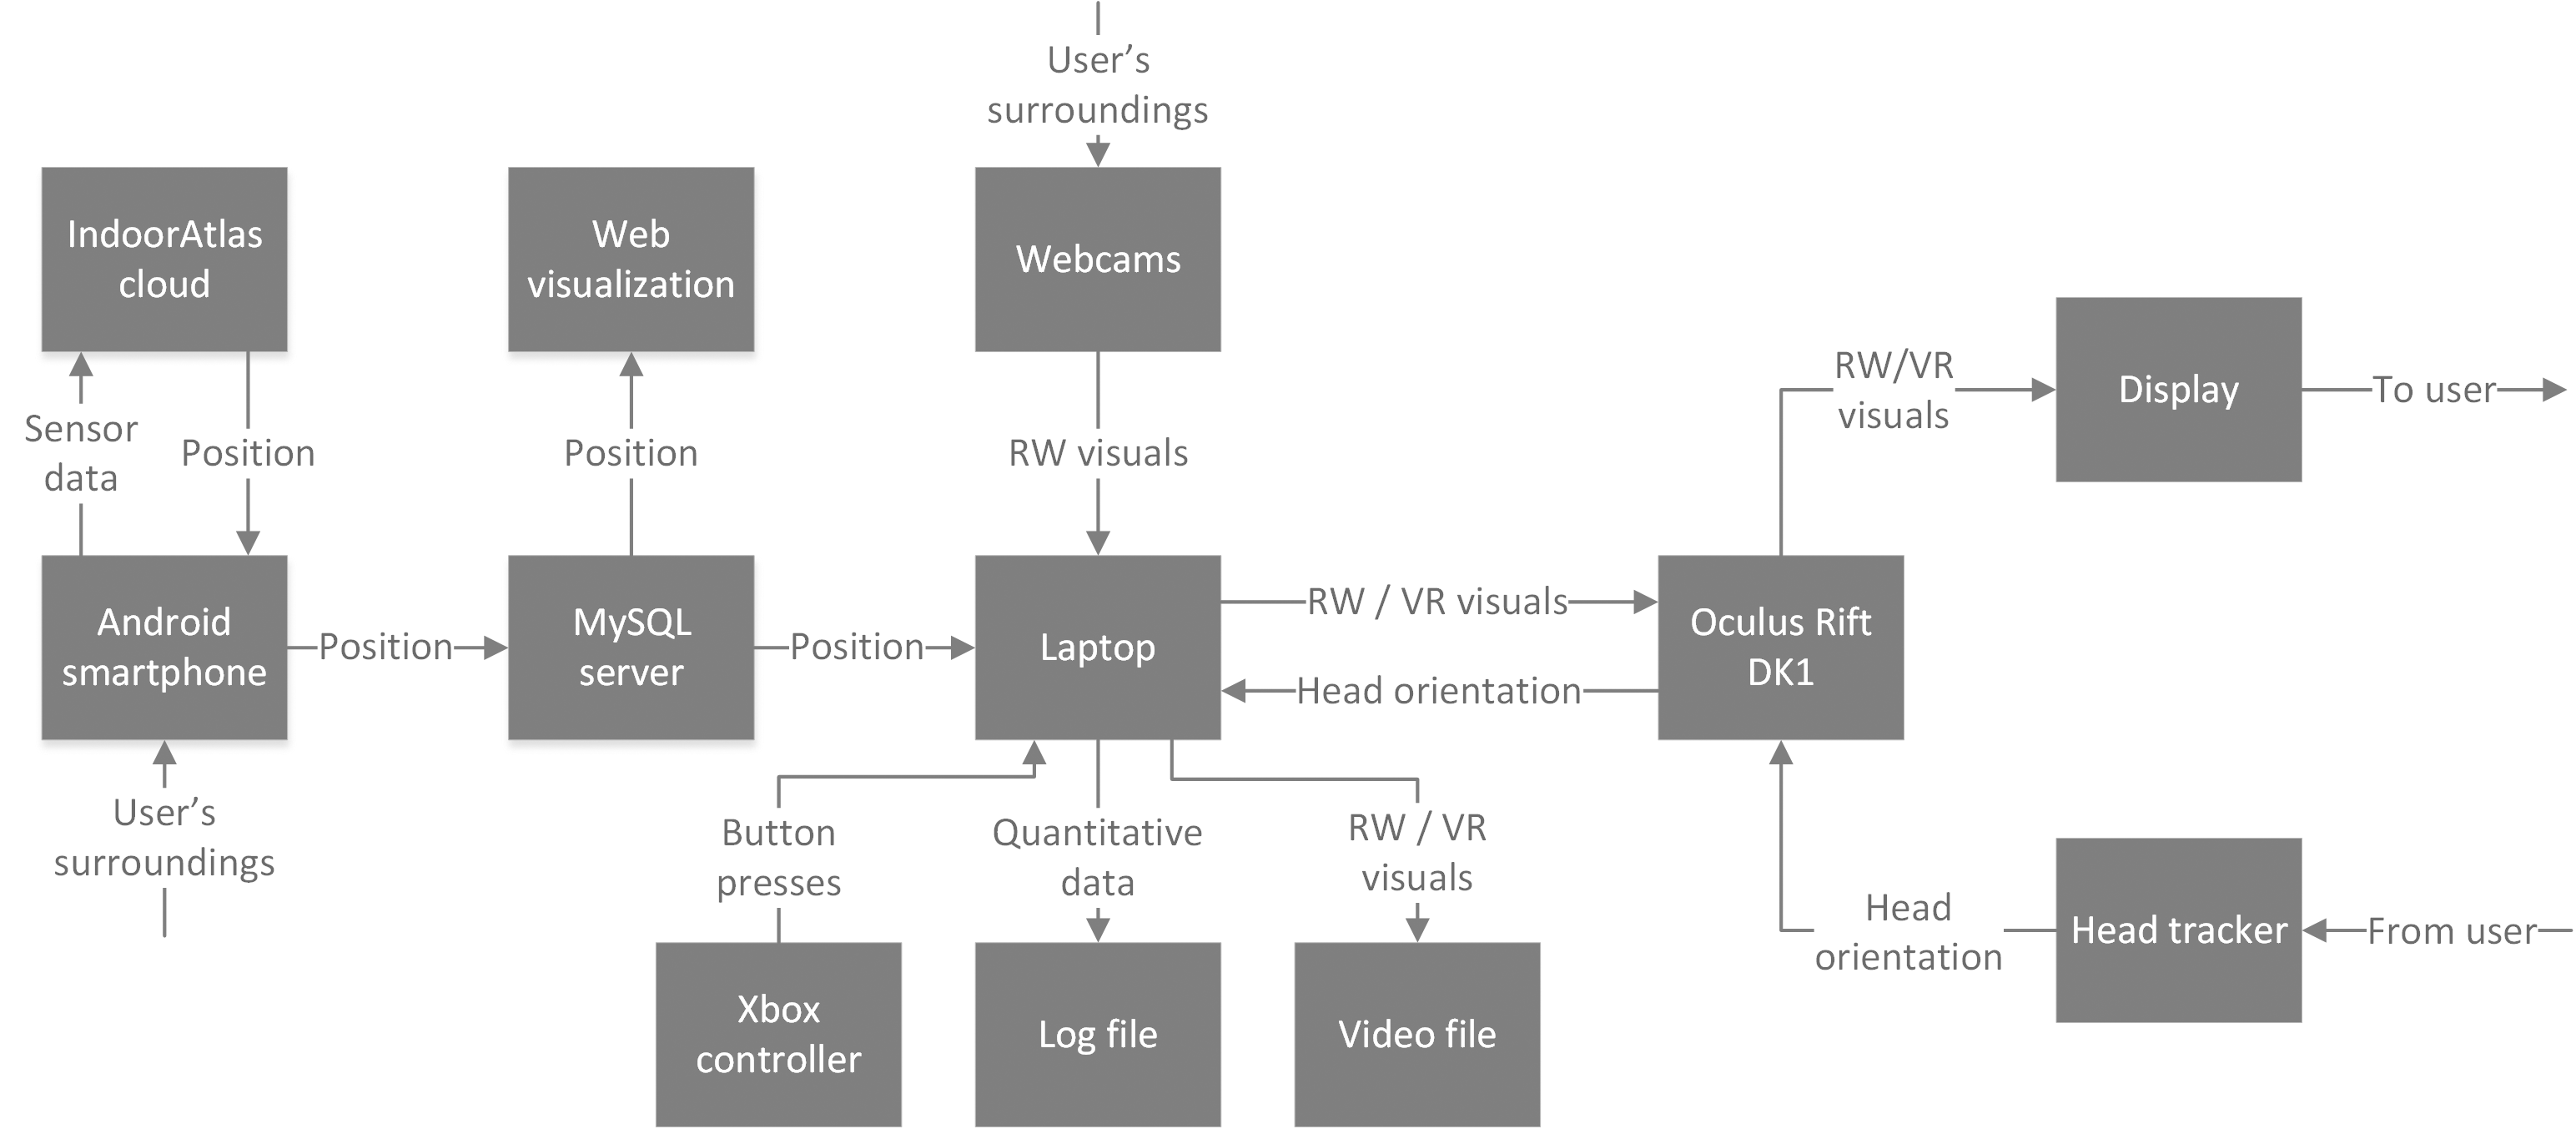
\includegraphics[width=.925\linewidth]{experimental-implementation.png}
		\caption{Implementation of Mirrorshades platform.}
		\label{experimentalimplementation}
	\end{center}
\end{figure}

%=========================================================================================================

\subsection{Hardware Components}
The hardware of the implementation comprises;

\begin{itemize}
	\item an Oculus Rift DK1 HMD, including a 9-axis (3dof rotational) head tracker sampling at 1000Hz \& mounted with a stereo camera solution comprising 2x Logitech C310 webcams modified with M12 lens mounts \& 2.1mm lenses to provide approximately 87 degrees horizontal FOV of the RW environment (see figure \ref{rift});
	\item a USB battery pack, to power the HMD;
	\item a small laptop computer, with an Intel i7-3632QM processor, Nvidia GT 650M graphics card \& 16GiB system memory;
	\item an Android smartphone, running Android 4.4.4;
	\item an Xbox 360 wireless controller, with USB receiver.
\end{itemize}

%\begin{figure}[h]
%	\begin{center}
%		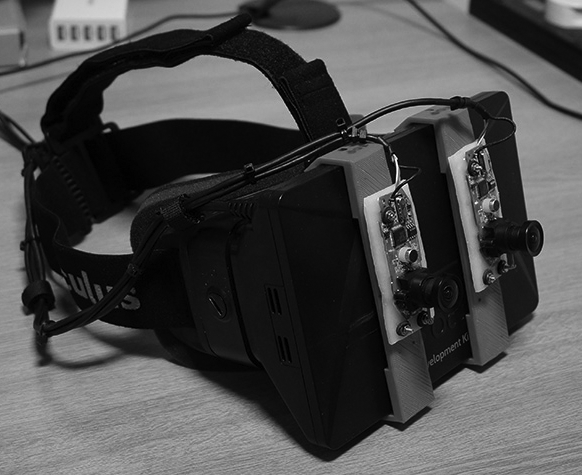
\includegraphics[width=0.6\textwidth]{rift.png}
%		\caption{HMD with stereo camera solution.}
%		\label{rift}
%	\end{center}
%\end{figure}

%=========================================================================================================

\subsection{Software Components}
The software of the implementation comprises;

\begin{itemize}
	\item an Android application that runs on the smartphone, determines the location of the phone within the building that it is in using the IndoorAtlas IPS~\cite{IndoorAtlasLtd.2012} (figure \ref{sallies_layout} shows the paths within the chapel upon which the IPS has been configured) \& submits these location data via PHP to a database server;
	\item a MySQL database server that stores location data for the phone \& allows these data to be accessed both by the Unity application running upon the laptop \& by a web visualisation;
	\item a Unity application that runs on the laptop.
\end{itemize}

%=========================================================================================================

\subsection{Integration of Components}
The Unity application hosts the VR representation of the chapel \& takes in feeds from both webcams, the HMD head tracker \& the Xbox controller. It also polls the database server for the most recent position data. All of these inputs are combined together to form the visual output for the HMD to display to the user.

As the user moves their head, the visuals that are presented to them upon the HMD's display change accordingly; the RW visuals change due to the webcams being physically fixed to the HMD \& the VR visuals change due to data from the head tracker being used to change the orientation of the in game `cameras' accordingly.

As the user changes their position by walking, the visuals that are presented to them upon the HMD's display also change accordingly; again the RW visuals change due to the webcams' position upon the HMD whilst the VR visuals change due to the user's position, as reported by the smartphone \& the IndoorAtlas solution, being used to move the position of the in game cameras to the equivalent position within the VR representation.

As the user presses buttons or pulls triggers upon the Xbox controller, the visuals that are presented to them upon the HMD's display transition between RW \& VR in different styles depending upon which button/trigger was activated.

%=========================================================================================================

\subsection{Transition Methods}
Attending to visual stimuli from the RW environment via the webcams is required for the user to safely move around. Delay in the IPS reporting their position \& inaccuracies in these position data (see figure \ref{jack-cole-splodges} for a set of example position data) mean that moving around while attending only to visual stimuli from the VR environment would not be safe for the user, even with unchanging RW obstacles with perfectly accurate representations in the VR environment. Furthermore it is actually likely that RW obstacles will not have equivalent VR representations, such as in a scenario where XR is used to compare \& contrast changes to a building's interior over extended periods of time (such as with the chapel investigations).

Thus the HMD displays the feeds from the webcams as default \& the user must trigger transitions to view the VR environment by pressing a button or pulling a trigger on the controller. Releasing the button/trigger causes the webcam feeds to be displayed again.

%=========================================================================================================

\subsubsection{Hard switch}
\label{sub-hardswitch}
The user presses \& holds the \texttt{[A]} button on the controller to switch the visual stimuli displayed by the HMD from RW to VR. When the \texttt{[A]} button is released, the visual stimuli displayed by the HMD switch back from VR to RW. This is a `hard' or `immediate' switch with no fading or transition effect. Figure \ref{scenario1} illustrates this scenario.

\begin{figure}[h]
	\begin{center}
		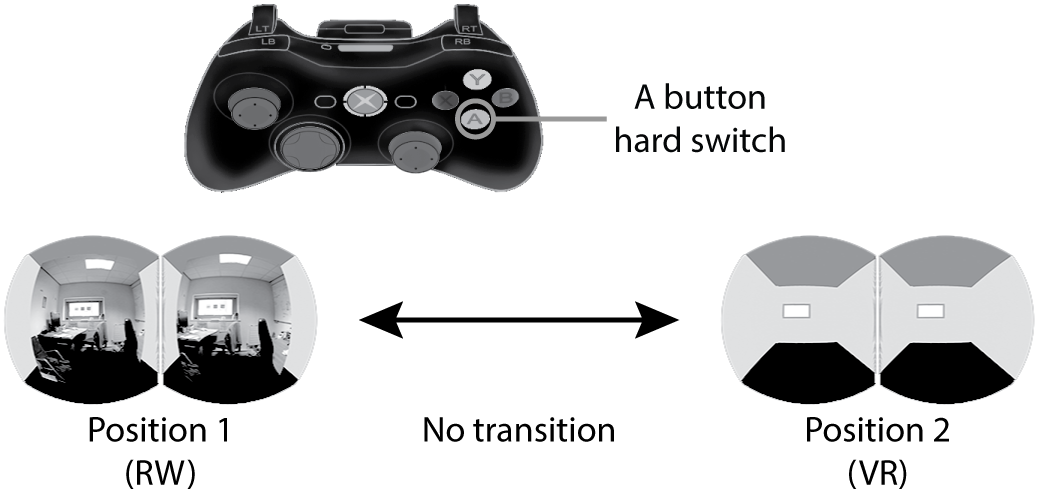
\includegraphics[width=0.7\textwidth]{switching-hard-with-controller.png}
		\caption{Hard switch.}
		\label{scenario1}
	\end{center}
\end{figure}

%=========================================================================================================

\subsubsection{Switch with linear interpolation}
The user presses \& holds the \texttt{[B]} button on the controller to switch the visual stimuli displayed by the HMD from RW to VR. When the \texttt{[B]} button is released, the visual stimuli displayed by the HMD switch back from VR to RW. This switch fades between RW \& VR  visual stimuli using linear interpolation on the opacity of the game objects that the webcam feeds are rendered upon. Figure \ref{scenario12} illustrates this scenario.

\begin{figure}[h]
	\begin{center}
		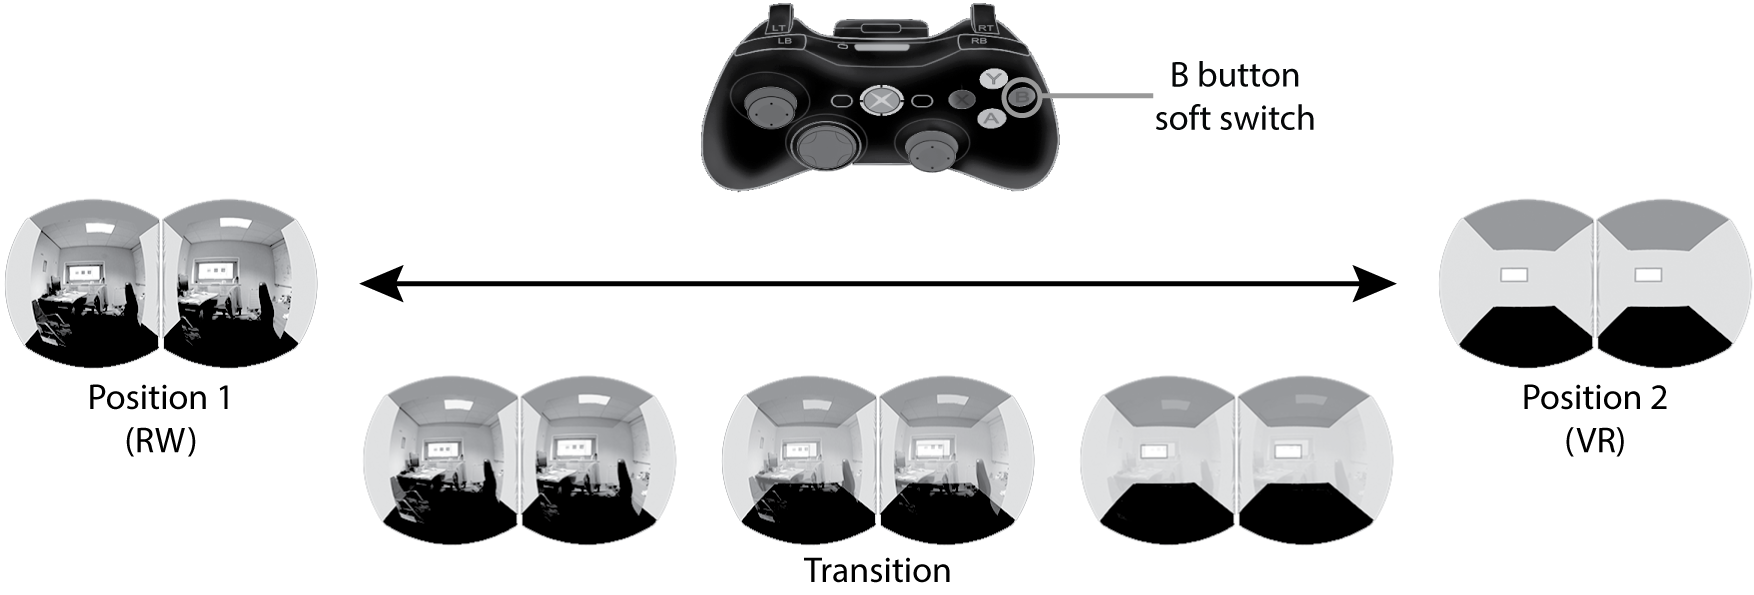
\includegraphics[width=\textwidth]{switching-soft-with-controller.png}
		\caption{Switch with linear interpolation.}
		\label{scenario12}
	\end{center}
\end{figure}

%=========================================================================================================

\subsubsection{Analogue selectable opacity}
The user pulls the right analogue trigger (\texttt{[RT]}) on the controller, where the position of the trigger maps directly to the opacity of the game objects that the webcam feeds are rendered upon. The user can choose to stop at any intermediary position that suits their needs, keeping the level of opacity of the webcam feeds at that position, as well as controlling the rate at which the visual stimuli from the RW environment fade (by changing how quickly they change their depression of the trigger). Pulling the trigger all the way in displays only visual stimuli from the VR environment, while releasing it completely displays only visual stimuli from the RW environment. The number of intermediary positions is limited only by the resolution of the trigger \& the encoding of the value.

This method allows the user to superimpose VR visual stimuli upon RW visual stimuli. This is similar, but not identical, to AR, as instead of displaying a small number of virtual objects upon the user's view of their RW environment, a complete VR environment is superimposed upon the user's view of their RW environment. Figure \ref{scenario2} illustrates this scenario.

\begin{figure}[h]
	\begin{center}
		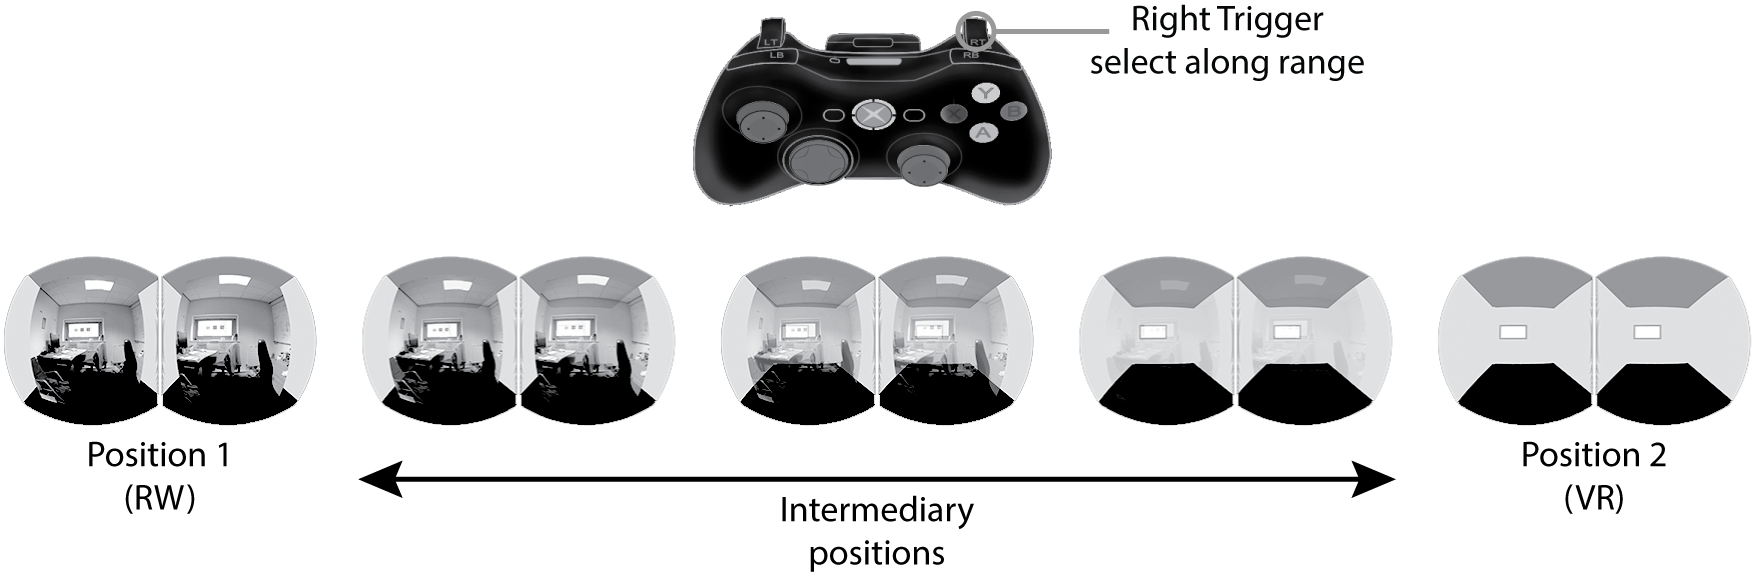
\includegraphics[width=.9\textwidth]{switching-analogue-with-controller.png}
		\caption{Analogue selectable opacity.}
		\label{scenario2}
	\end{center}
\end{figure}

%=========================================================================================================

\subsubsection{Periodic hard switches}
\label{subsub-periodic}
Independent or in addition to any of the previous scenarios, the visual stimuli displayed by the HMD switch from RW to VR at a set interval \& for a set amount of time. For example, every 3 seconds the stimuli switch from RW to VR for 0.2 of a second before switching back from VR to RW. Any user triggered transitions cause the interval timer to be reset, such that an `automated' switch will never occur after less time from a user triggered switch than the set interval. Automated transitions are disabled whilst \texttt{[RT]} is at all depressed. Figure \ref{scenariotimed} illustrates this scenario, where \texttt{i} represents the interval between switches \& \texttt{d} represents the duration of the switch from RW to VR.

\begin{figure}[h]
	\begin{center}
		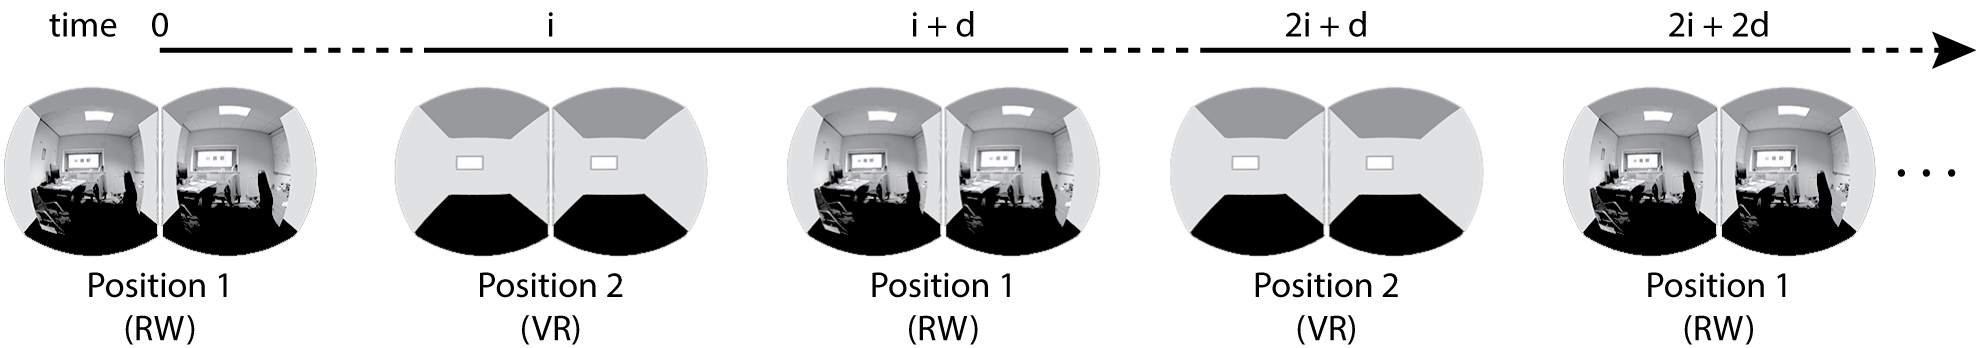
\includegraphics[width=\textwidth]{timed-switch.png}
		\caption{Periodic hard switches.}
		\label{scenariotimed}
	\end{center}
\end{figure}

%=========================================================================================================

\subsubsection{Reduced maximum opacity}
\label{subsub-baseopacity}
Independent or in addition to any of the previous scenarios, the maximum opacity of the game objects that the webcam feeds are rendered upon is reduced, such that the `default' position at which a transition has not been triggered (either by a button press, trigger movement or by a periodic switch) displays VR superimposed upon RW. Figure \ref{scenariobaseopacity} illustrates this scenario in combination with a hard switch (from section \ref{sub-hardswitch}) in which the user triggers hard switches between the default position of a superimposition of VR upon RW \& a position where only VR stimuli are present.

\begin{figure}[h]
	\begin{center}
		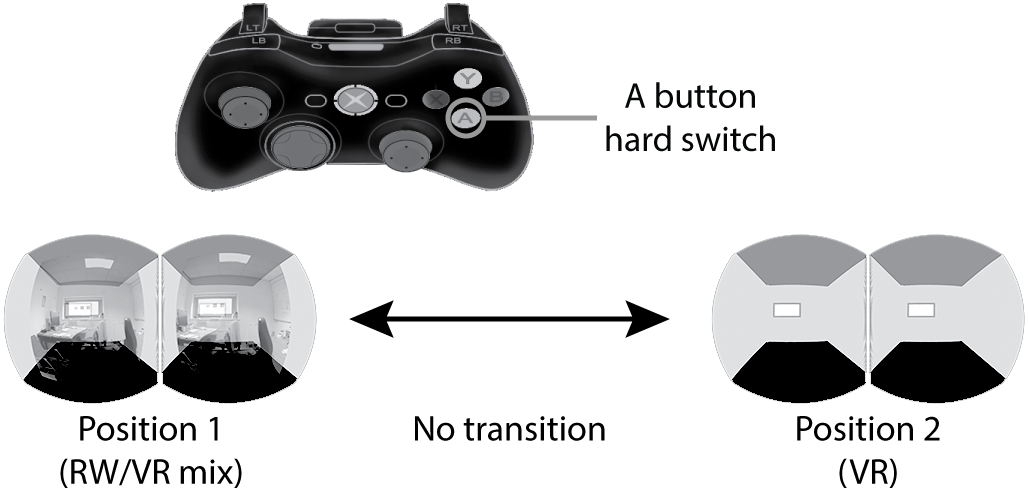
\includegraphics[width=0.7\textwidth]{base-opacity-hard-switch.png}
		\caption{Hard switch from reduced maximum opacity.}
		\label{scenariobaseopacity}
	\end{center}
\end{figure}

%=========================================================================================================





















%=========================================================================================================

%\textit{Two different buildings have been prepared for use with the Mirrorshades platform, with VR environments constructed \& the IndoorAtlas IPS deployed. The first is a modern building accompanied by a VR environment that closely depicts it in the present day. The second is a historic building accompanied by a VR environment that differs markedly from the present day, by depicting its state a point hundreds of years in the past.}

%\textit{In the first, participants will be given a simple task to complete which will encourage them to engage with the VR environment even though it presents a similar view to their RW environment. In the second scenario, participants will be prompted to engage in more free form exploration of their environments, comparing \& contrasting the markedly different VR environment with what they see around them in their RW environment.}

%\subsection{Jack Cole Building}
%The School of Computer Science Jack Cole building at St Andrews is a modern building, built in 2004. The VR environment accompanying the building is a fairly close representation of the building as it stands today. Figure \ref{jc_layout} shows the layout of the building \& the path that IndoorAtlas has been prepared for.

%There are four coloured panels (red, green, blue \& yellow) situated within the VR building upon walls, floor \& ceiling. Participants will be asked to remember in what order these panels are seen as they walk a lap of the building. This task is designed to encourage participants to switch between RW \& VR visual stimuli, even though the VR visual stimuli are very similar to those of the RW environment. This scenario is also intended to encourage participants to keep moving, rather than stopping at \& starting.

%\begin{figure}[h]
%	\begin{center}
%		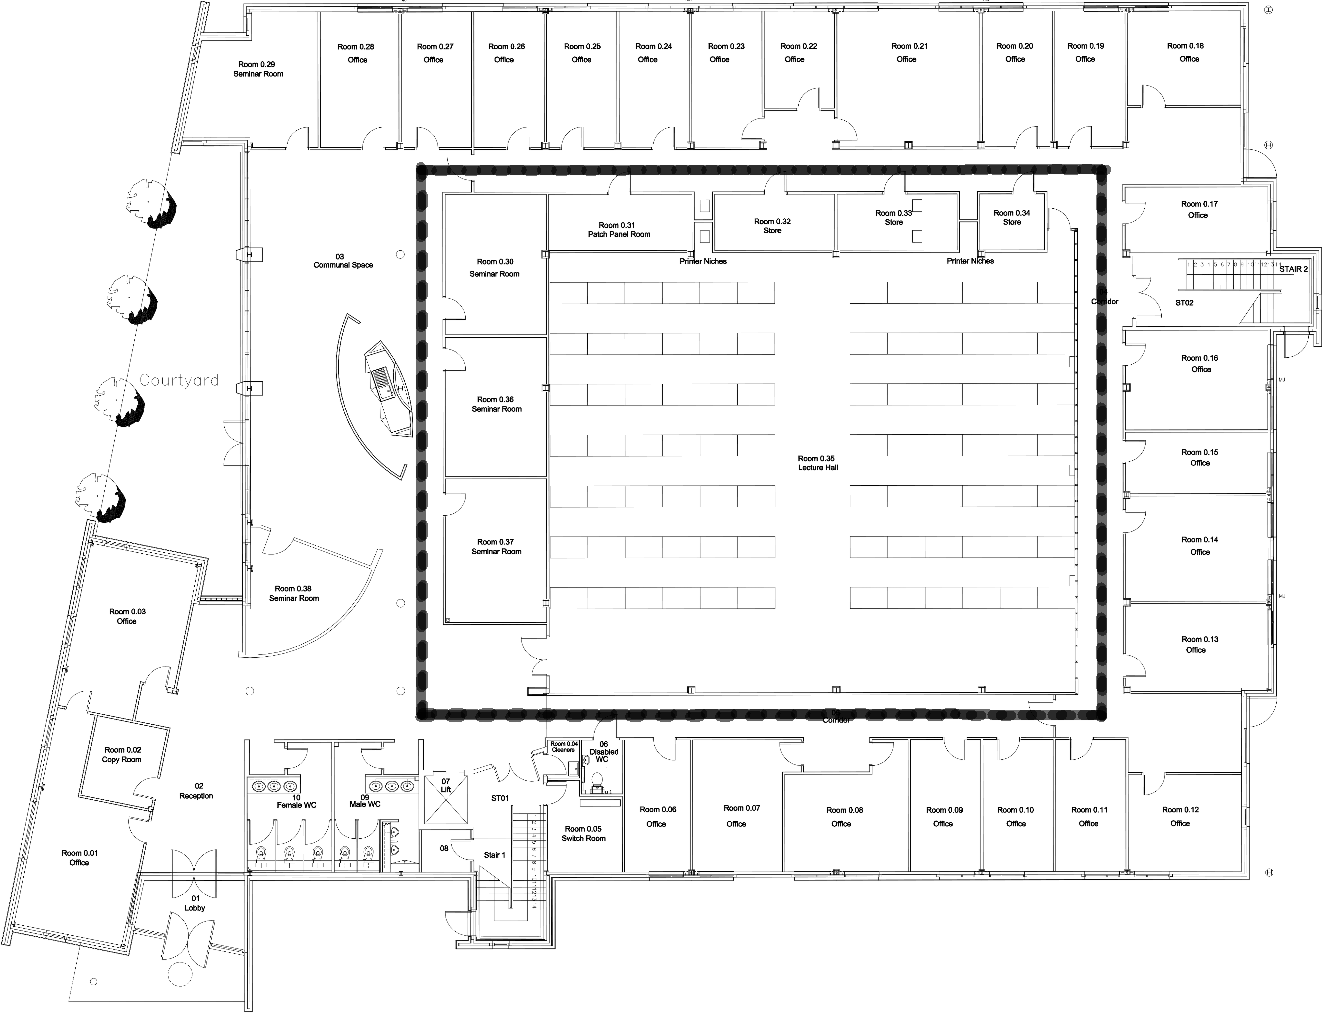
\includegraphics[width=0.7\textwidth]{JC_layout.png}
%		\caption{Floor plan of Jack Cole building, with IPS route.}
%		\label{jc_layout}
%	\end{center}
%\end{figure}

%=========================================================================================================